\documentclass[a4paper,10pt]{article}
\usepackage[utf8]{inputenc}
\usepackage{graphicx}

%opening
\title{}
\author{}

\begin{document}

\maketitle

\section{GE1LE0}
\graphicspath{{./GE1LE0PT2/}}
\begin{figure}[!ht]
\caption{Product Threshold 2}
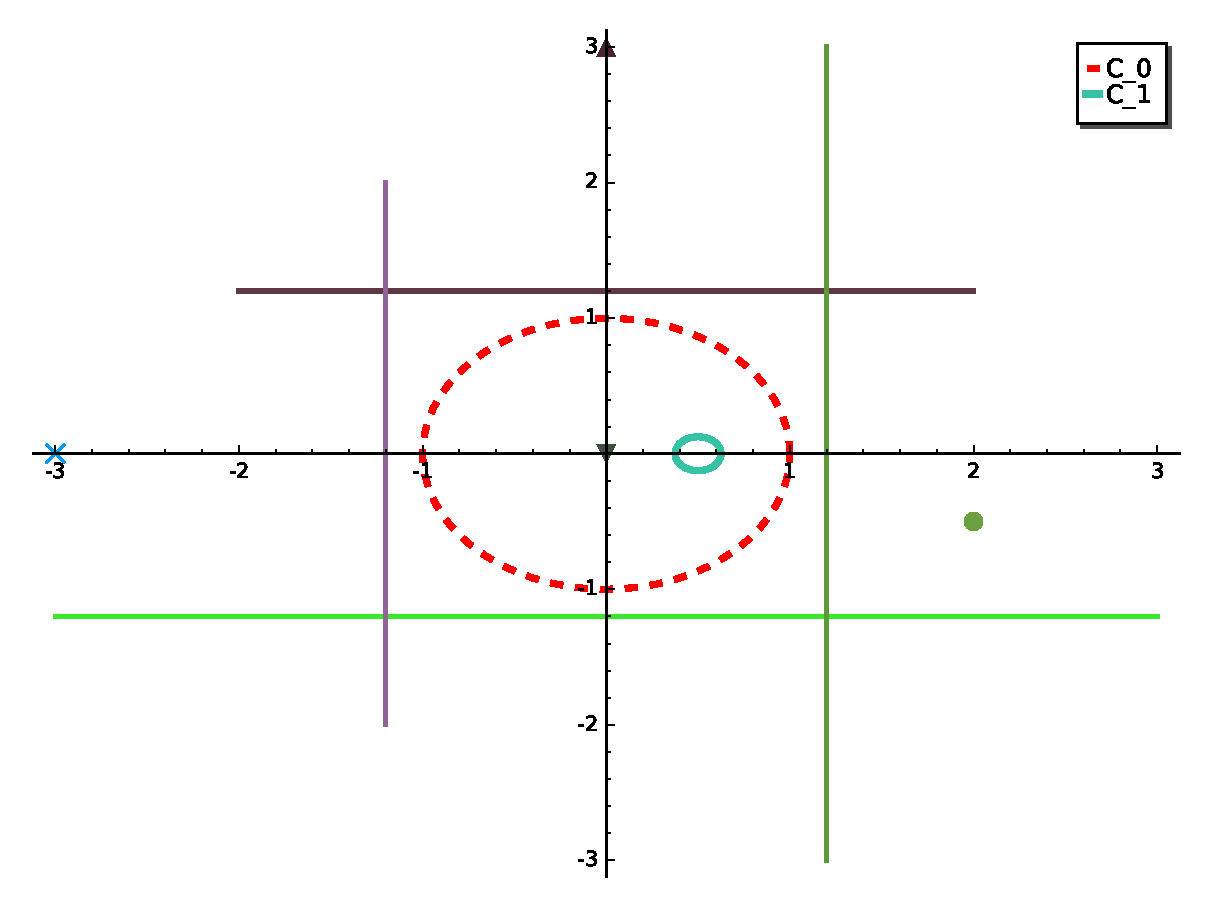
\includegraphics[width=0.5\textwidth]{circle_plot.eps}
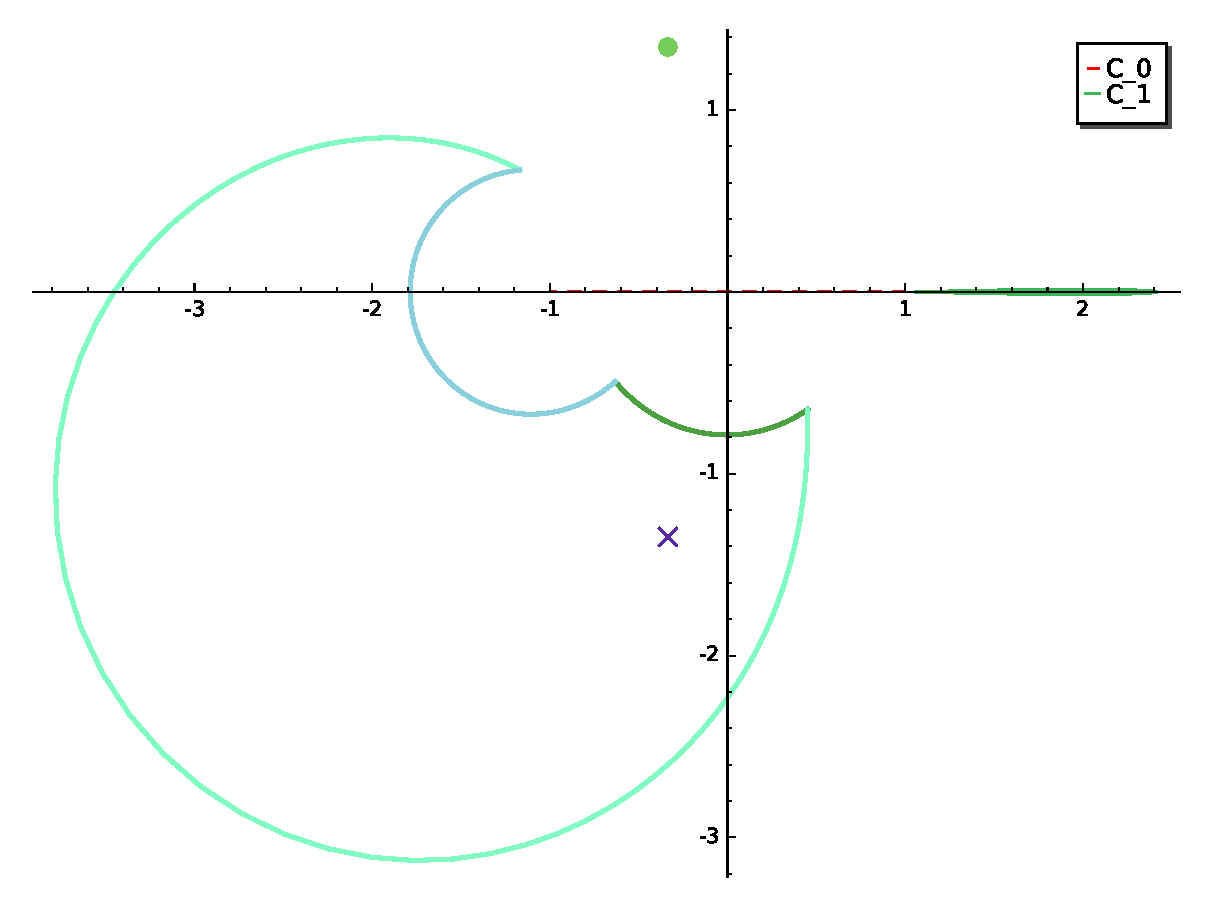
\includegraphics[width=0.5\textwidth]{zedplot.eps}
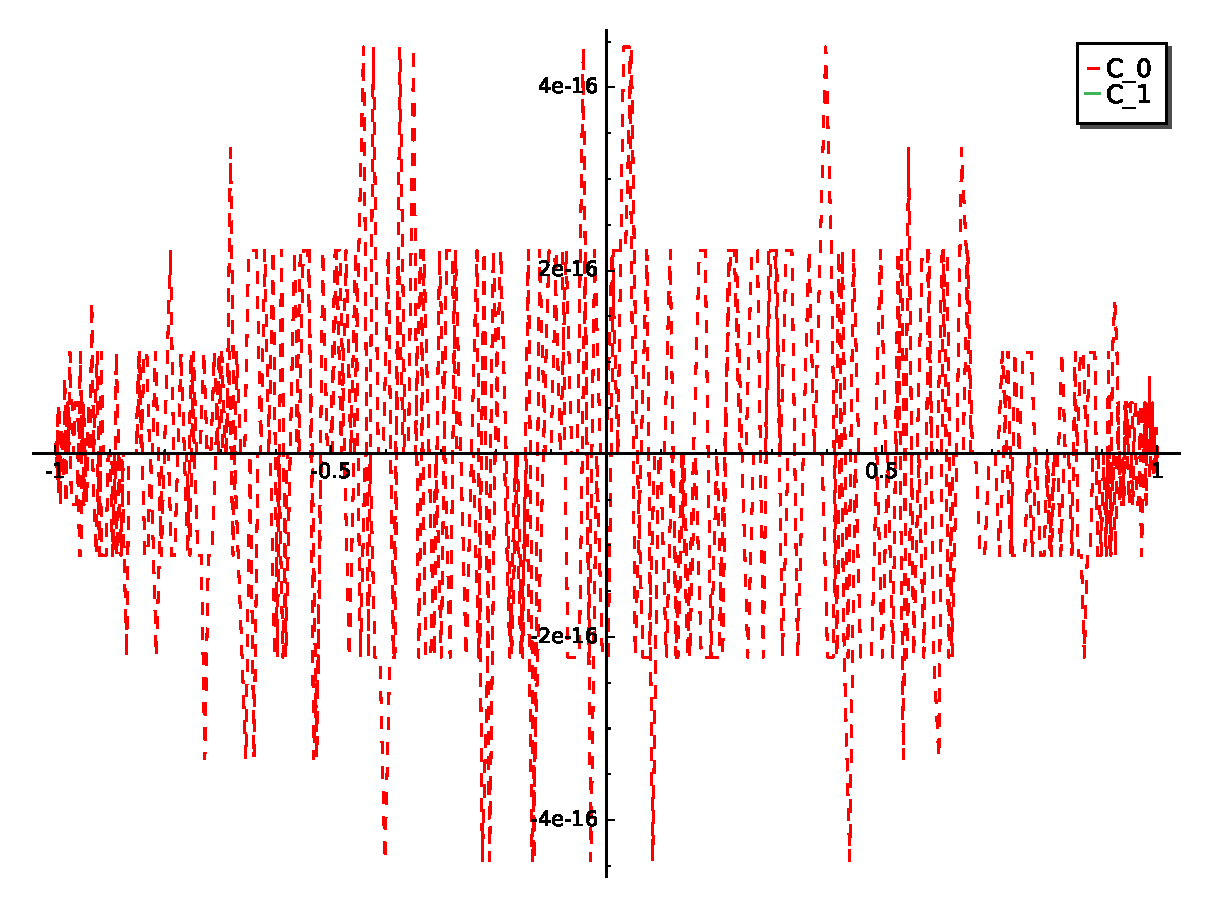
\includegraphics[width=0.5\textwidth]{zedplot_C0.eps}
\end{figure}

\graphicspath{{./GE1LE0PT3/}}
\begin{figure}
\caption{Product Threshold 3}
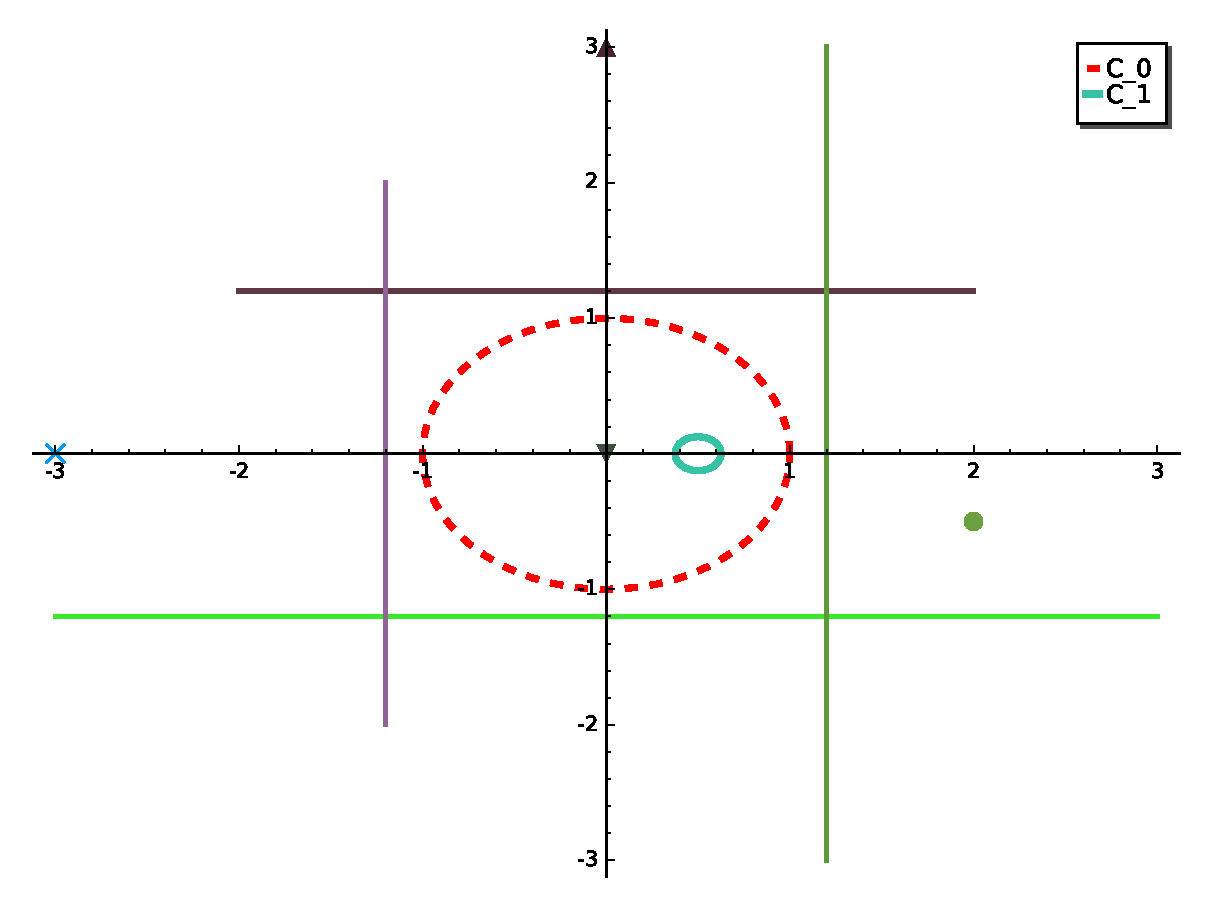
\includegraphics[width=0.5\textwidth]{circle_plot.eps}
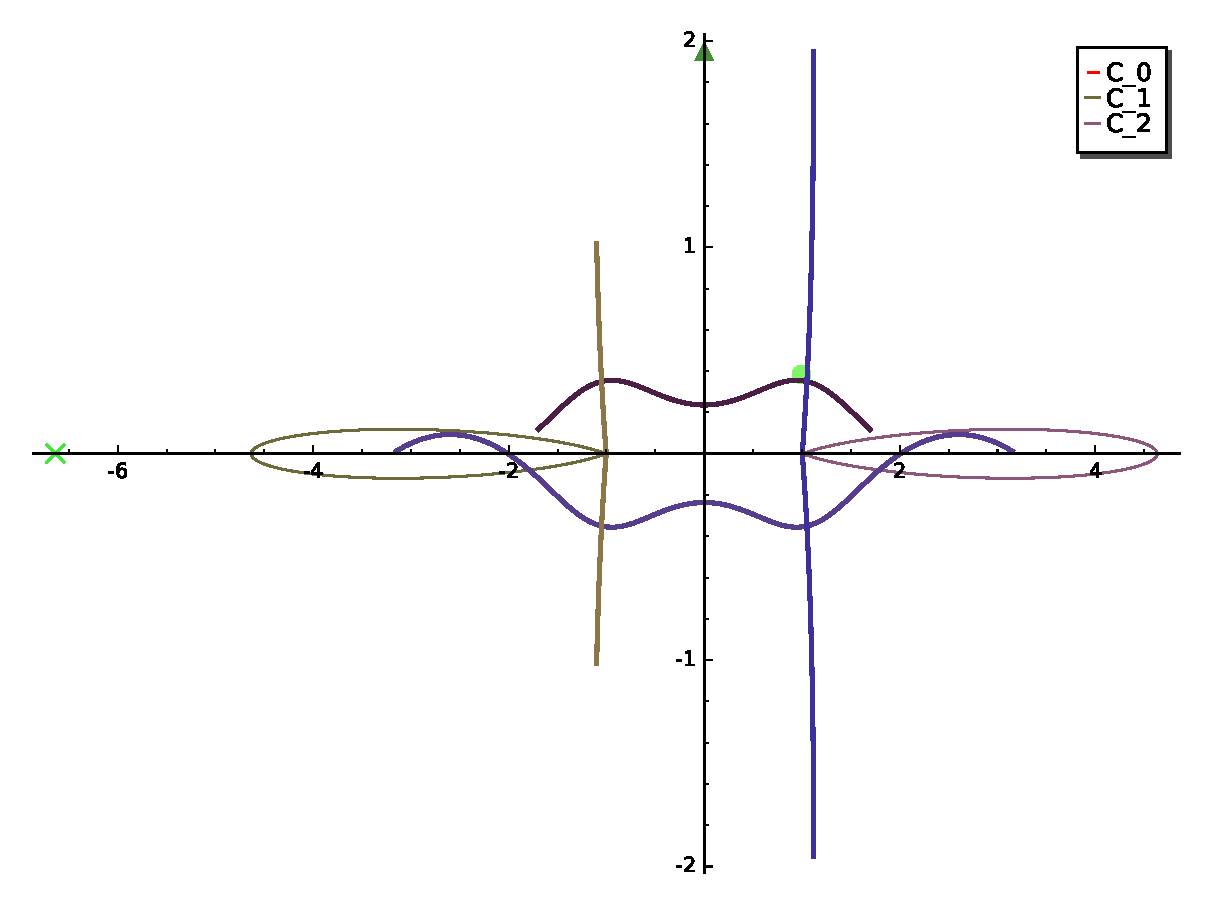
\includegraphics[width=0.5\textwidth]{zedplot.eps}
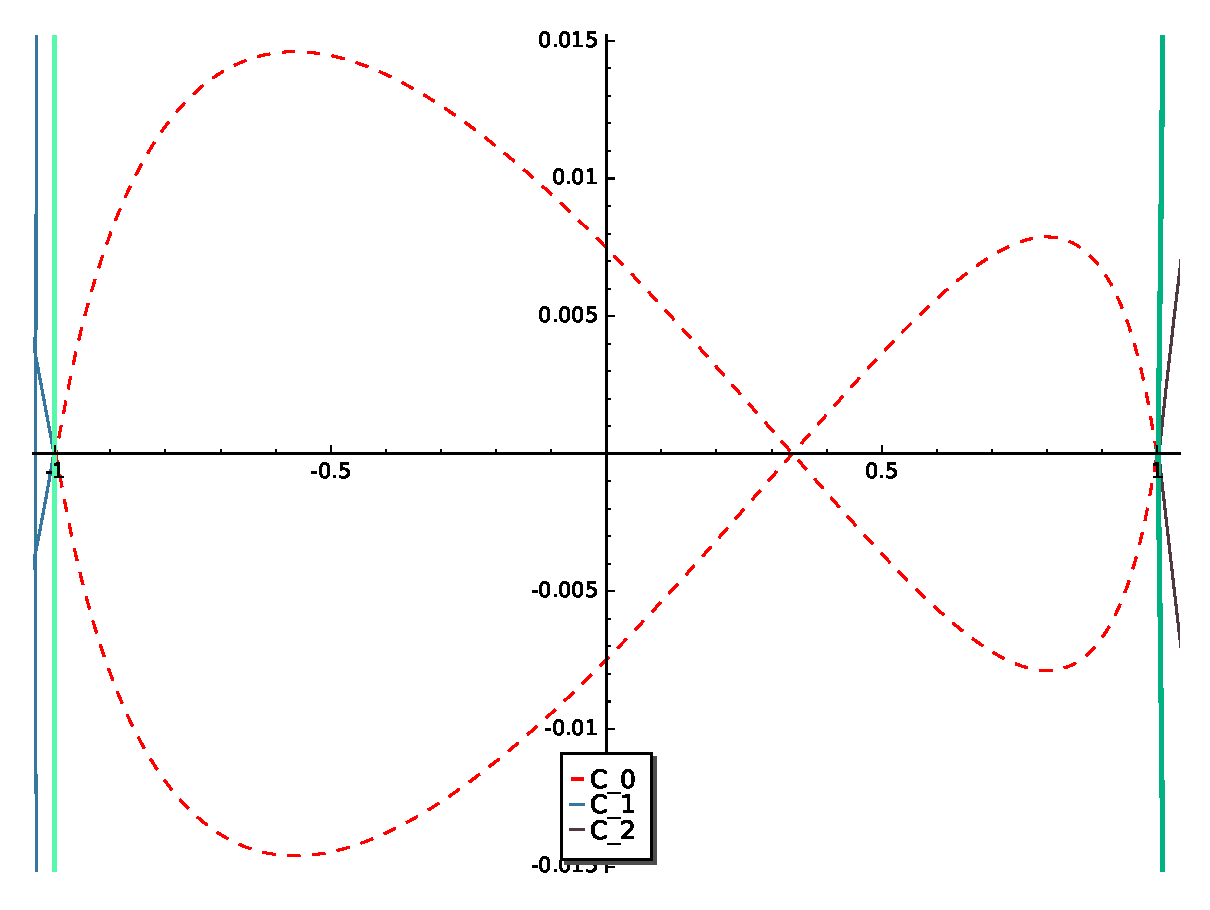
\includegraphics[width=0.5\textwidth]{zedplot_C0.eps}
\end{figure}

\graphicspath{{./GE1LE0PT4/}}
\begin{figure}
\caption{Product Threshold 4}
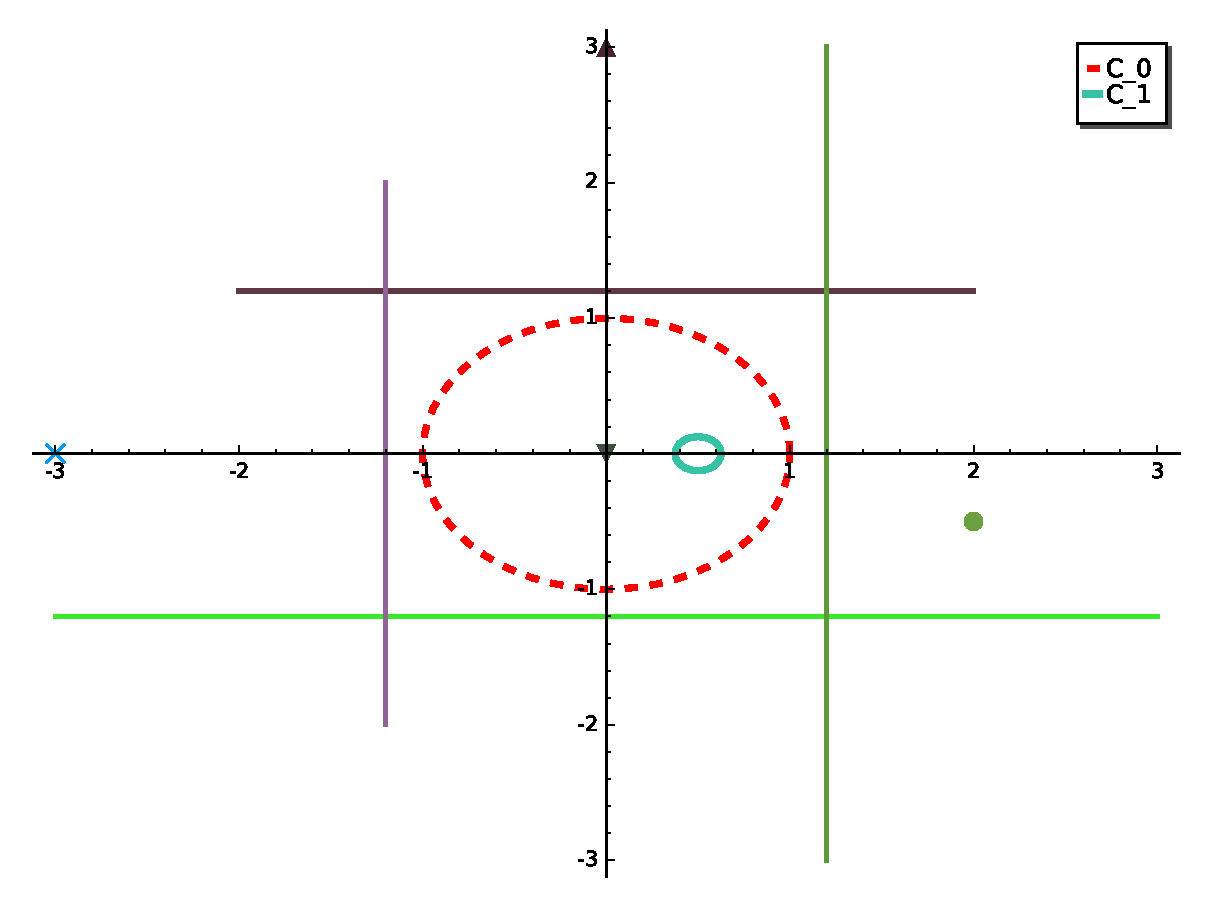
\includegraphics[width=0.5\textwidth]{circle_plot.eps}
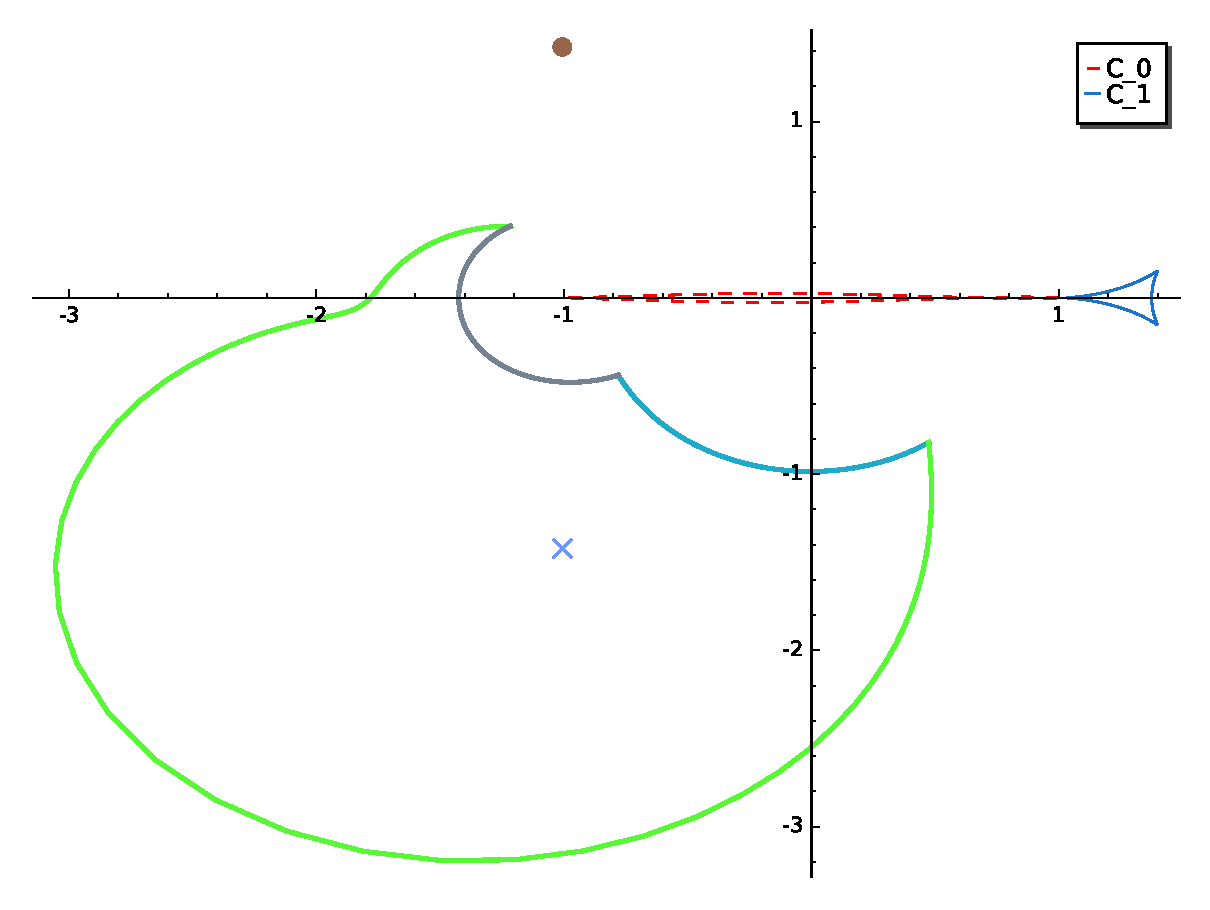
\includegraphics[width=0.5\textwidth]{zedplot.eps}
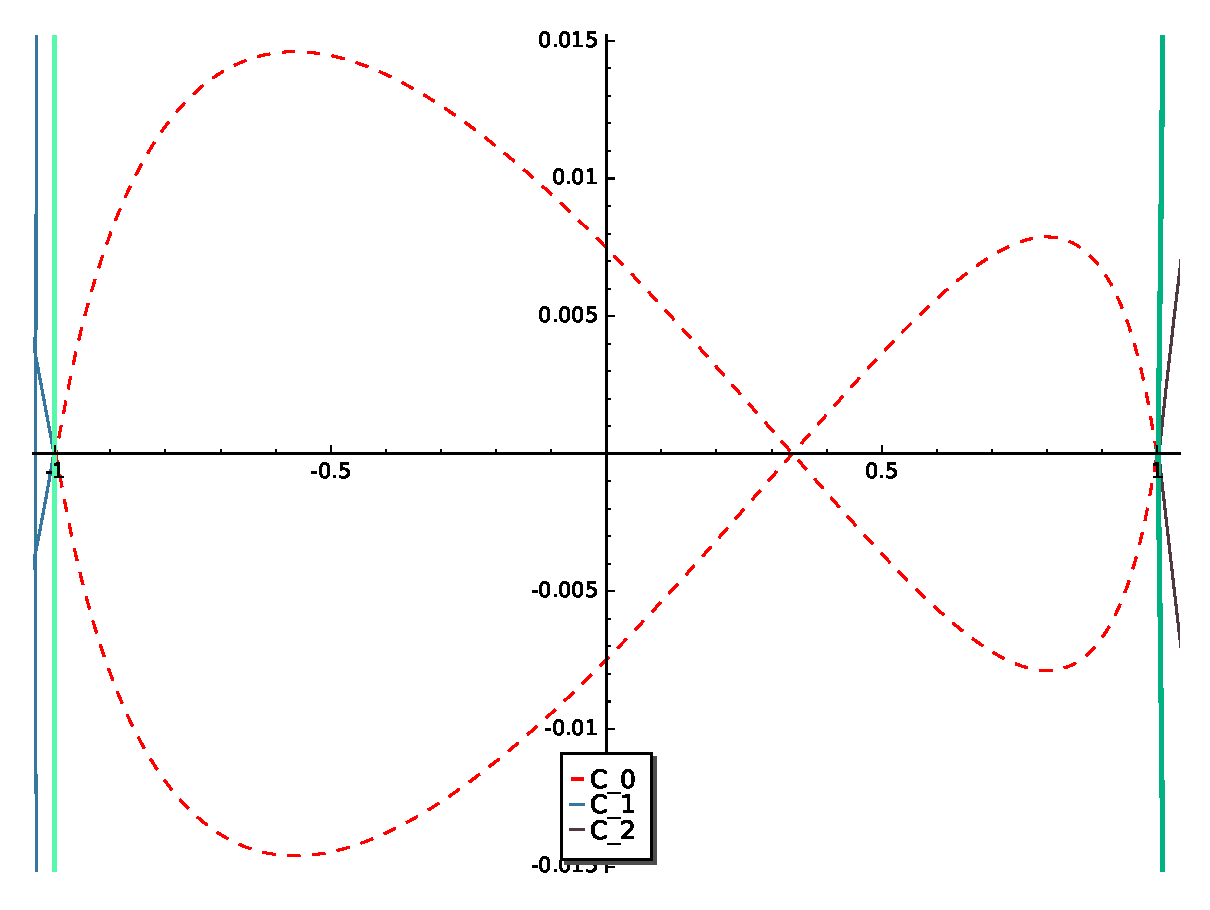
\includegraphics[width=0.5\textwidth]{zedplot_C0.eps}
\end{figure}

\graphicspath{{./GE1LE0PT5/}}
\begin{figure}
\caption{Product Threshold 5}
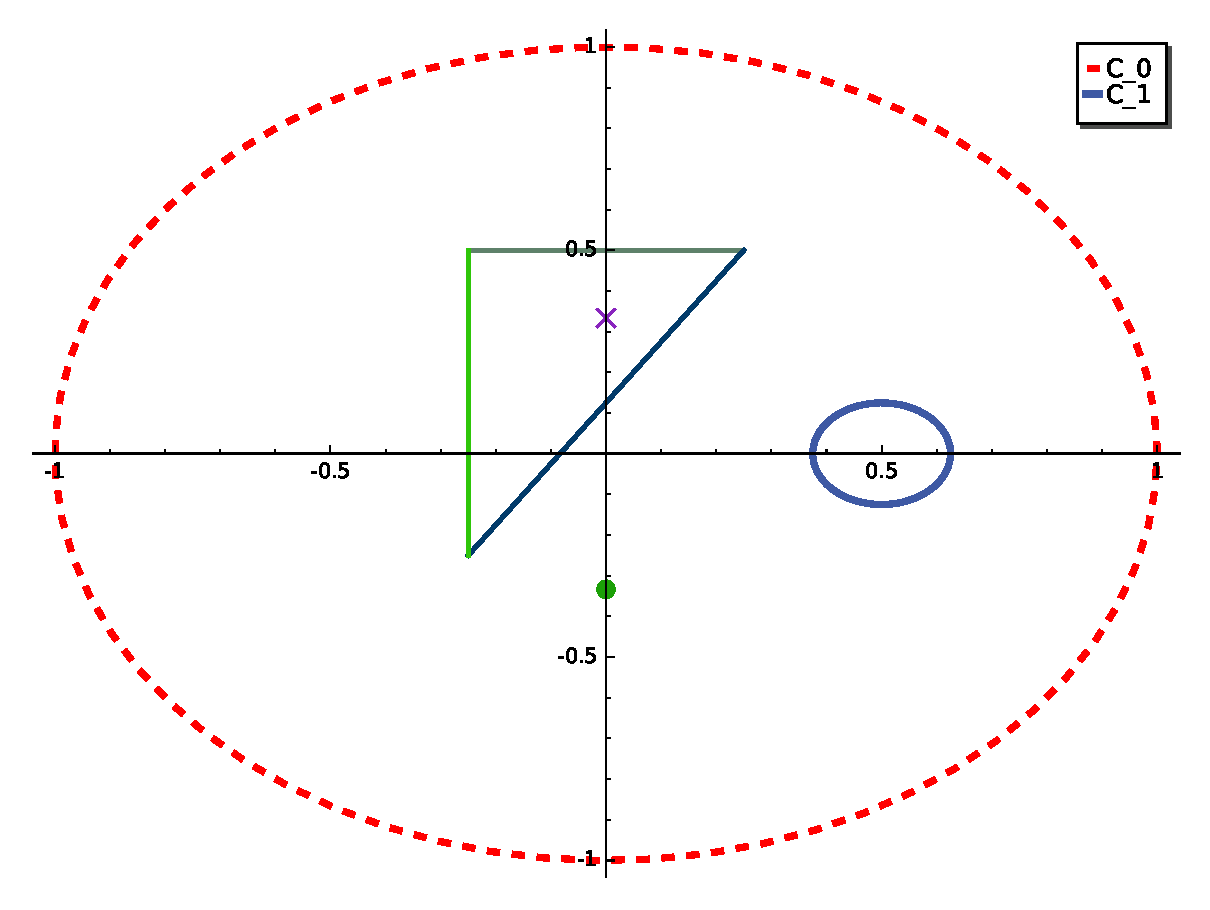
\includegraphics[width=0.5\textwidth]{circle_plot.eps}
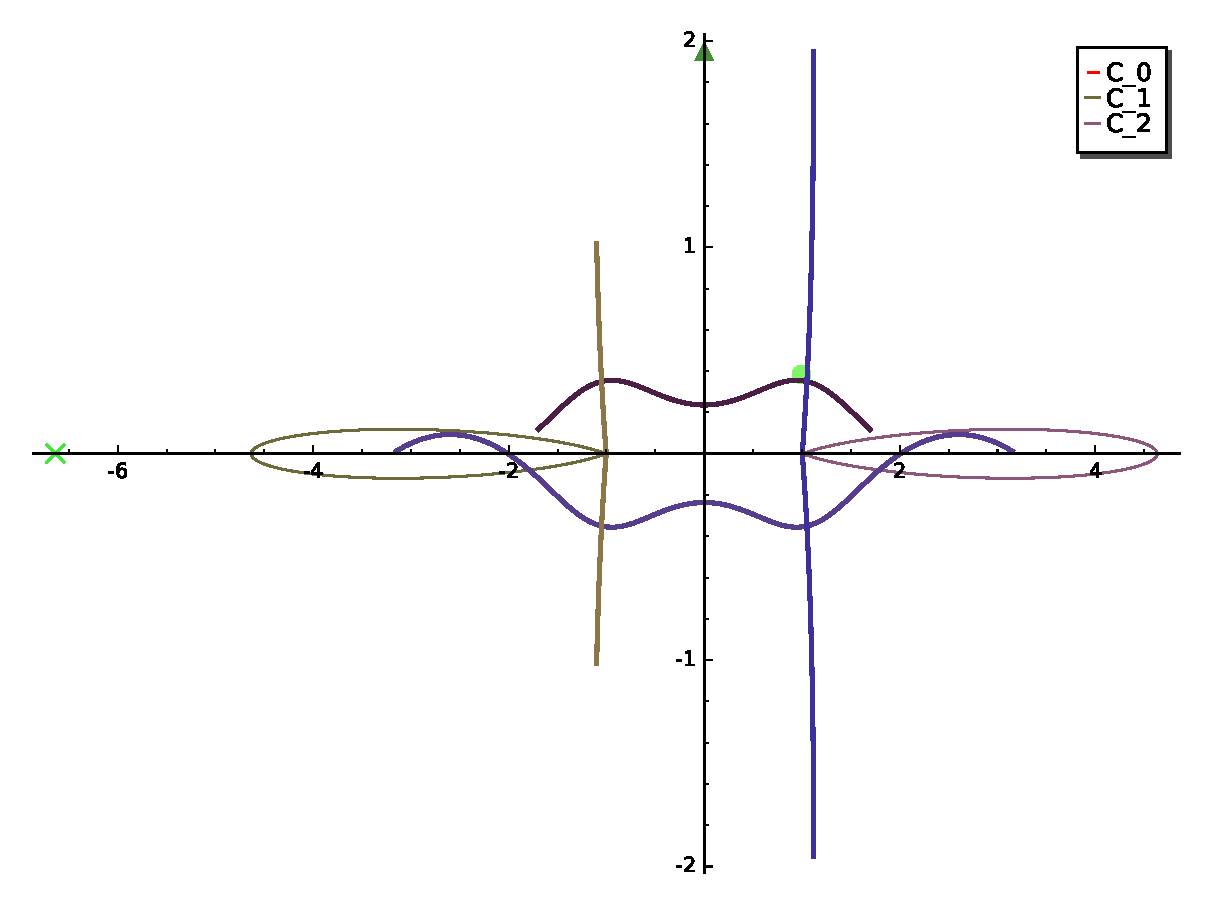
\includegraphics[width=0.5\textwidth]{zedplot.eps}
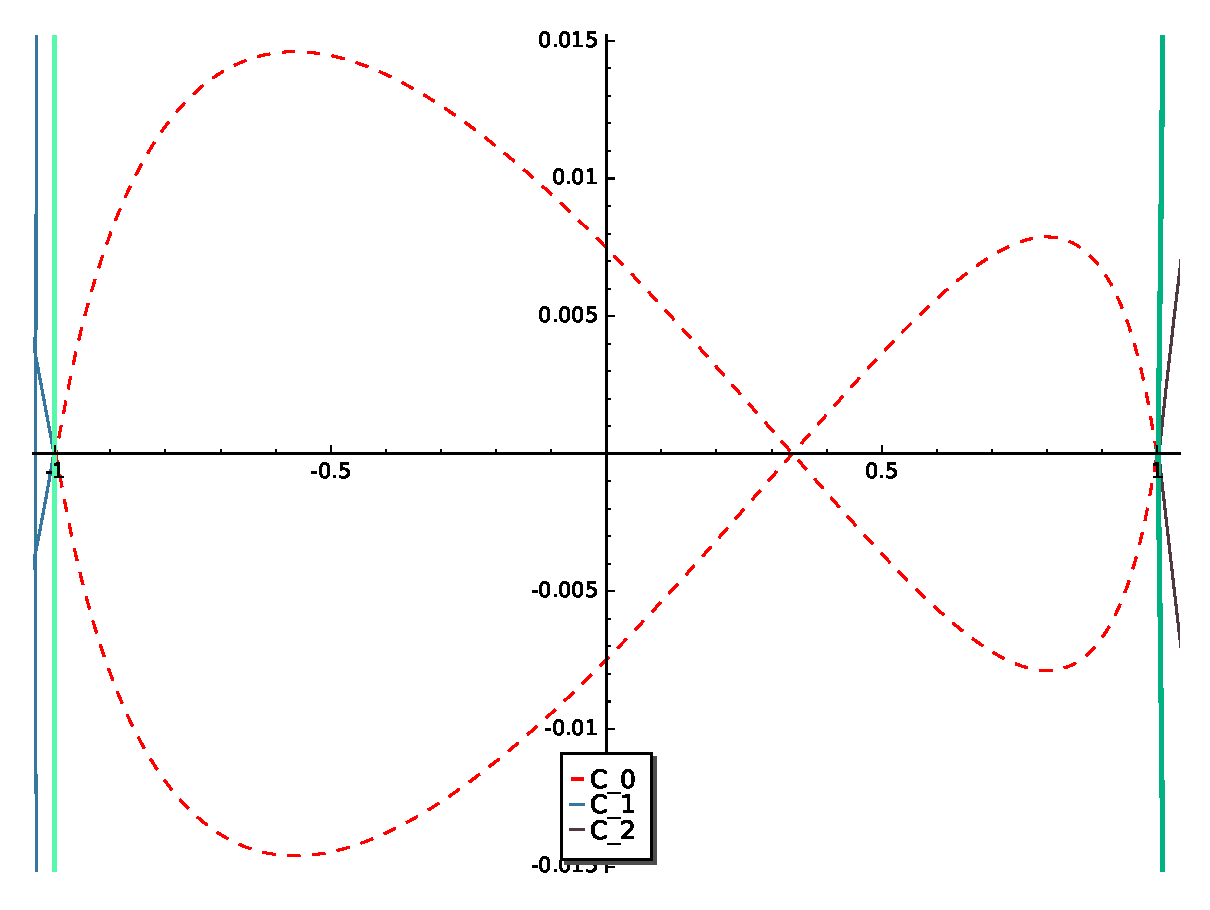
\includegraphics[width=0.5\textwidth]{zedplot_C0.eps}
\end{figure}


\newpage 
\clearpage
\section{GE1LE2}
\graphicspath{{./GE1LE2PT3/}}
\begin{figure}[!ht]
\caption{Product Threshold 3}
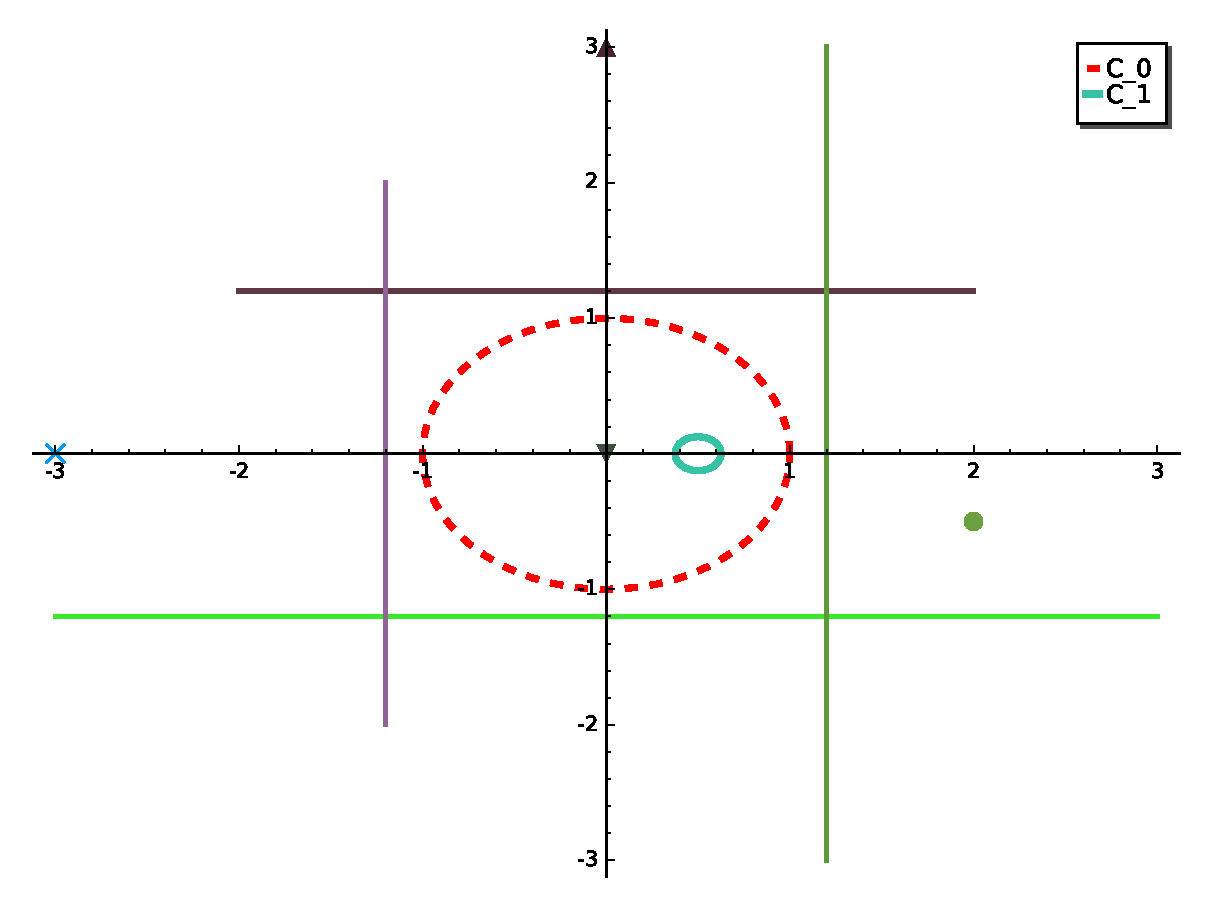
\includegraphics[width=0.5\textwidth]{circle_plot.eps}
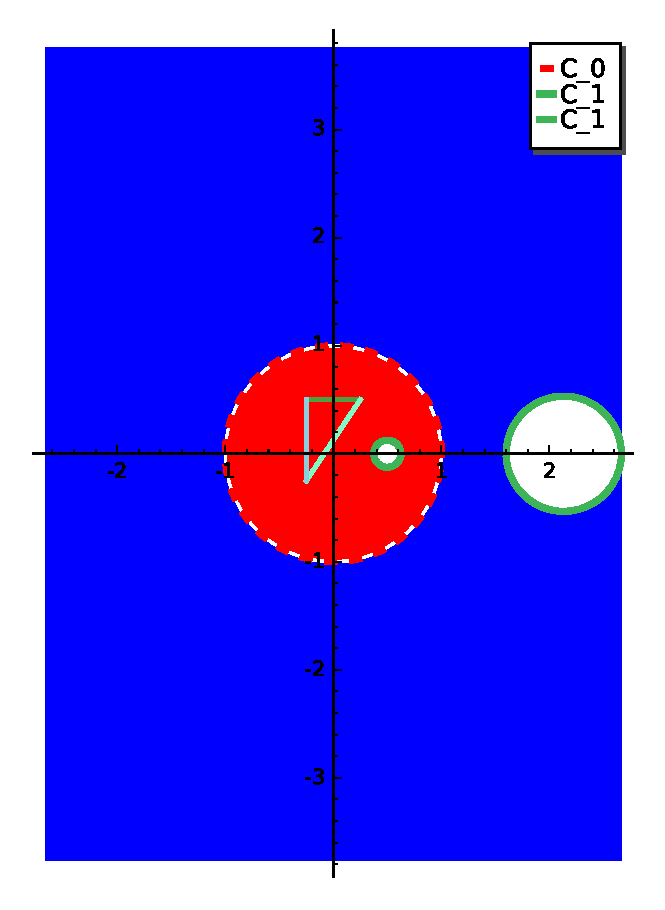
\includegraphics[width=0.5\textwidth]{Fundamental_domain.eps}
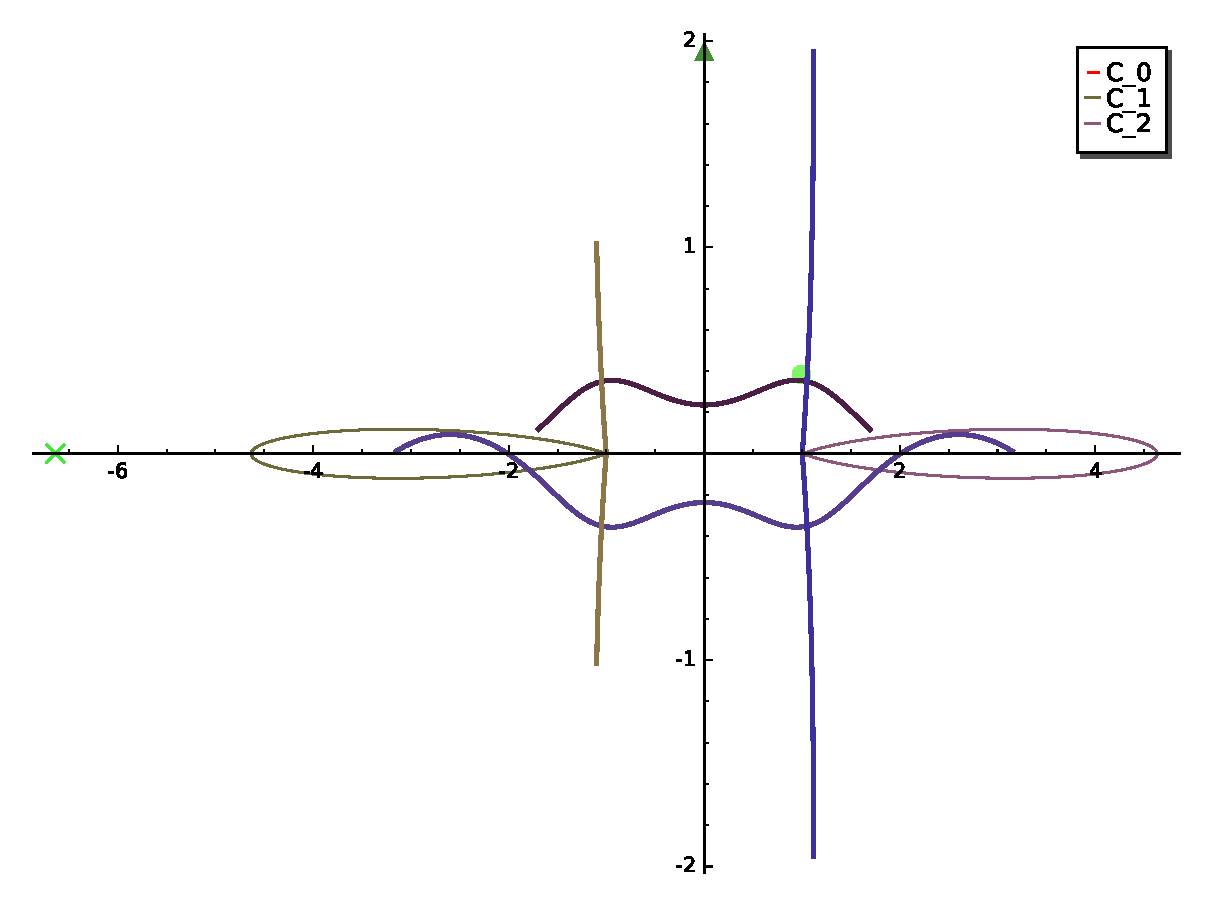
\includegraphics[width=0.5\textwidth]{zedplot.eps}
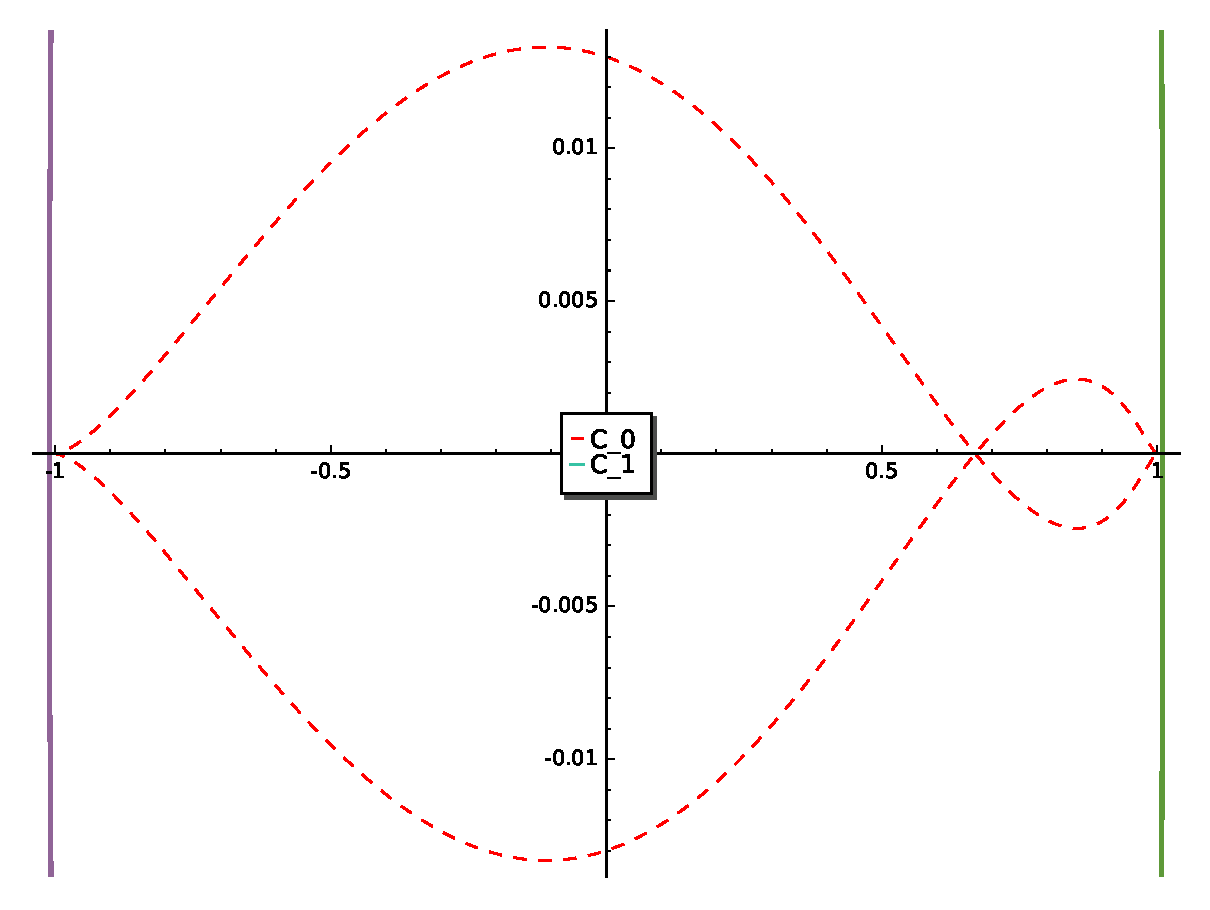
\includegraphics[width=0.5\textwidth]{zedplot_C0.eps}
\end{figure}

\graphicspath{{./GE1LE2PT4/}}
\begin{figure}
\caption{Product Threshold 4}
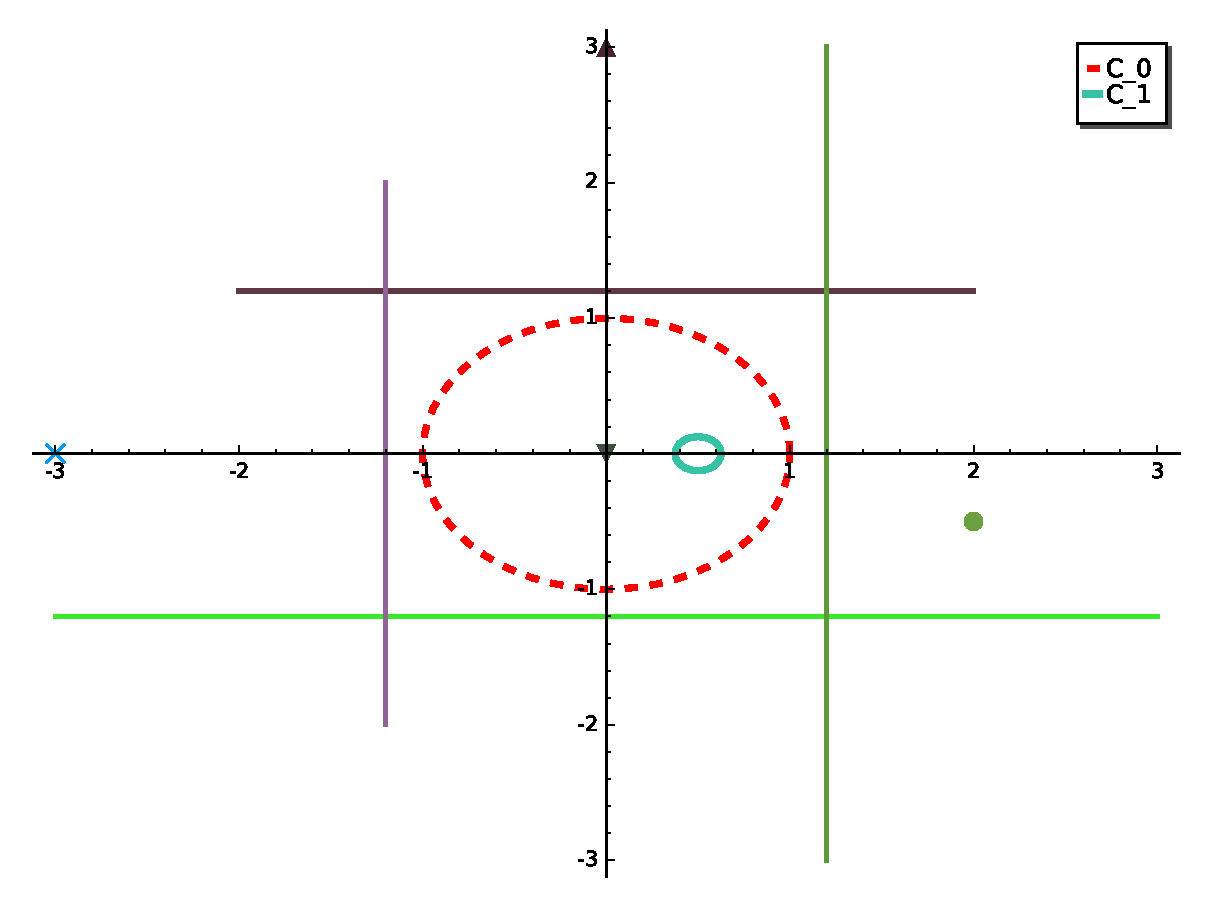
\includegraphics[width=0.5\textwidth]{circle_plot.eps}
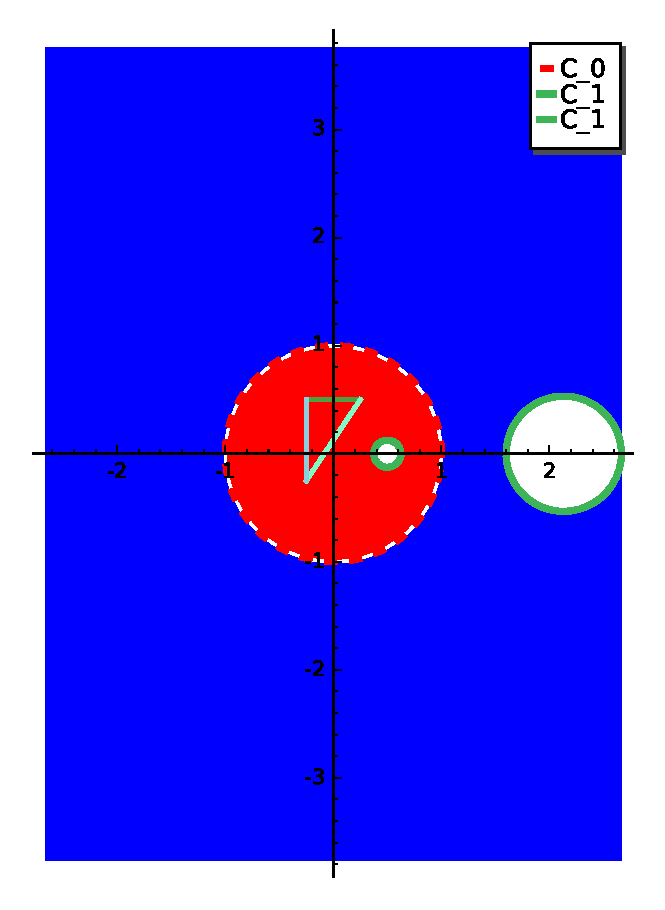
\includegraphics[width=0.5\textwidth]{Fundamental_domain.eps}
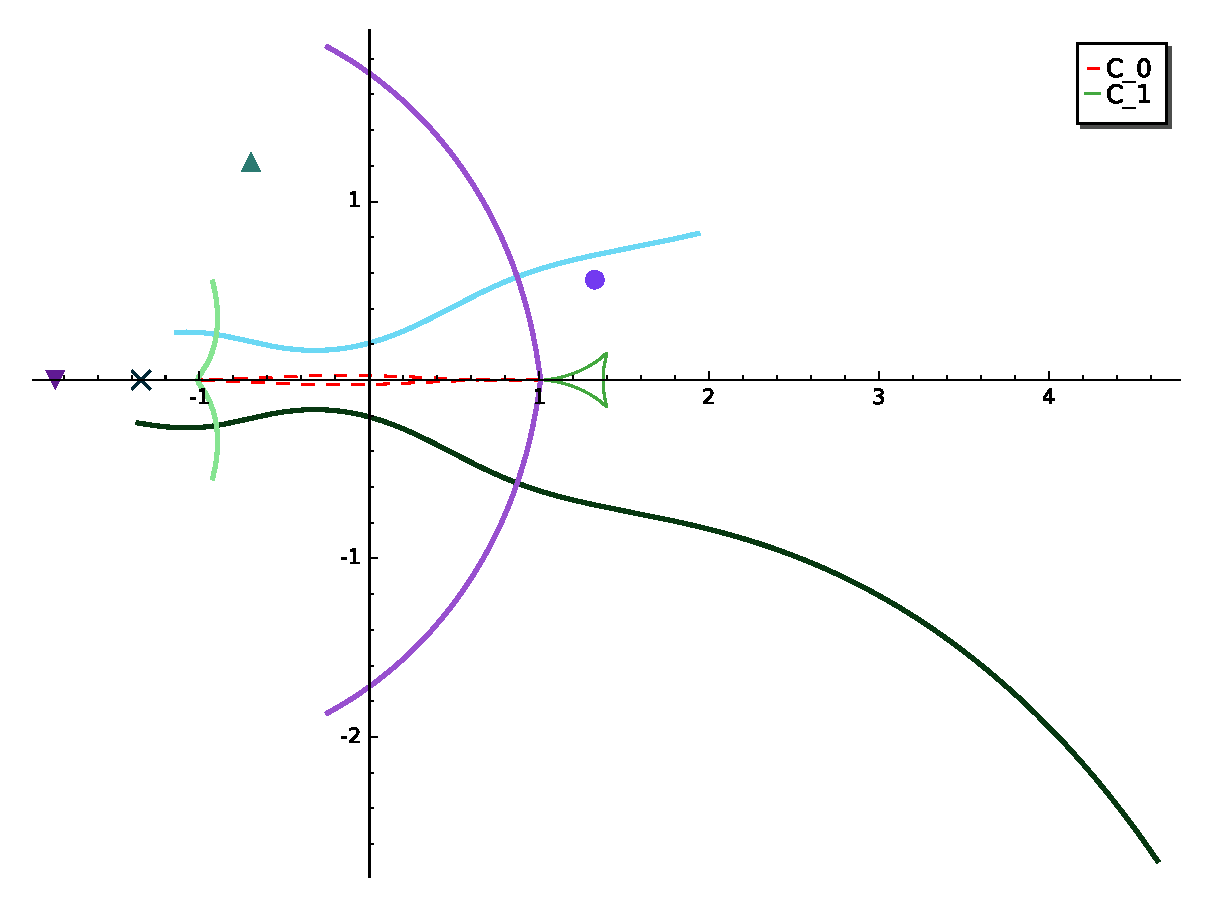
\includegraphics[width=0.5\textwidth]{zedplot.eps}
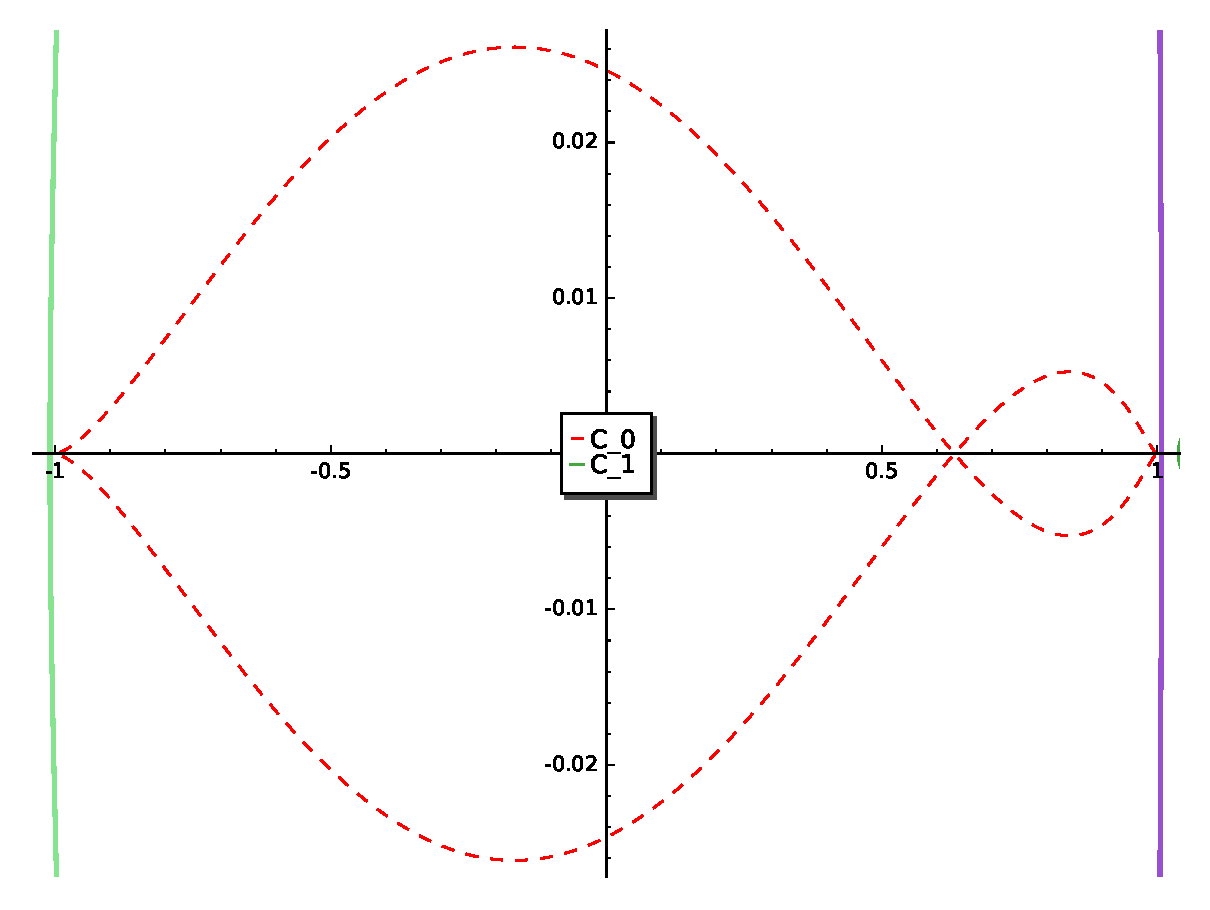
\includegraphics[width=0.5\textwidth]{zedplot_C0.eps}
\end{figure}

\graphicspath{{./GE1LE2PT5/}}
\begin{figure}
\caption{Product Threshold 5}
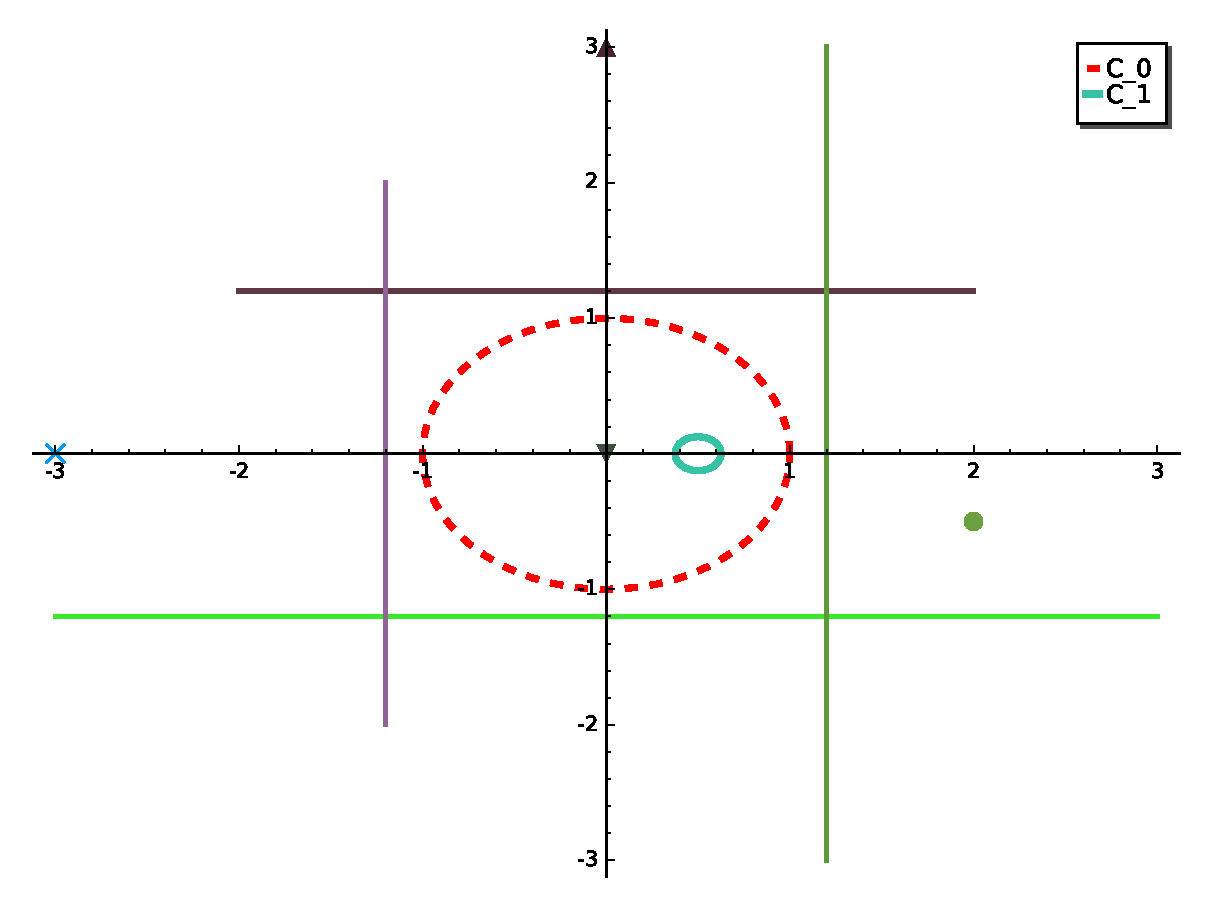
\includegraphics[width=0.5\textwidth]{circle_plot.eps}
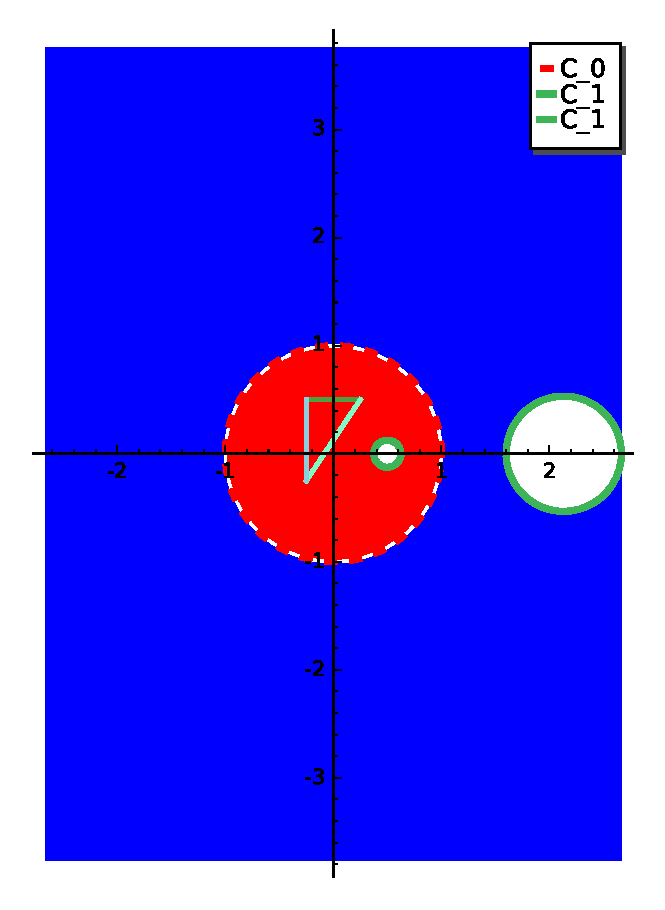
\includegraphics[width=0.5\textwidth]{Fundamental_domain.eps}
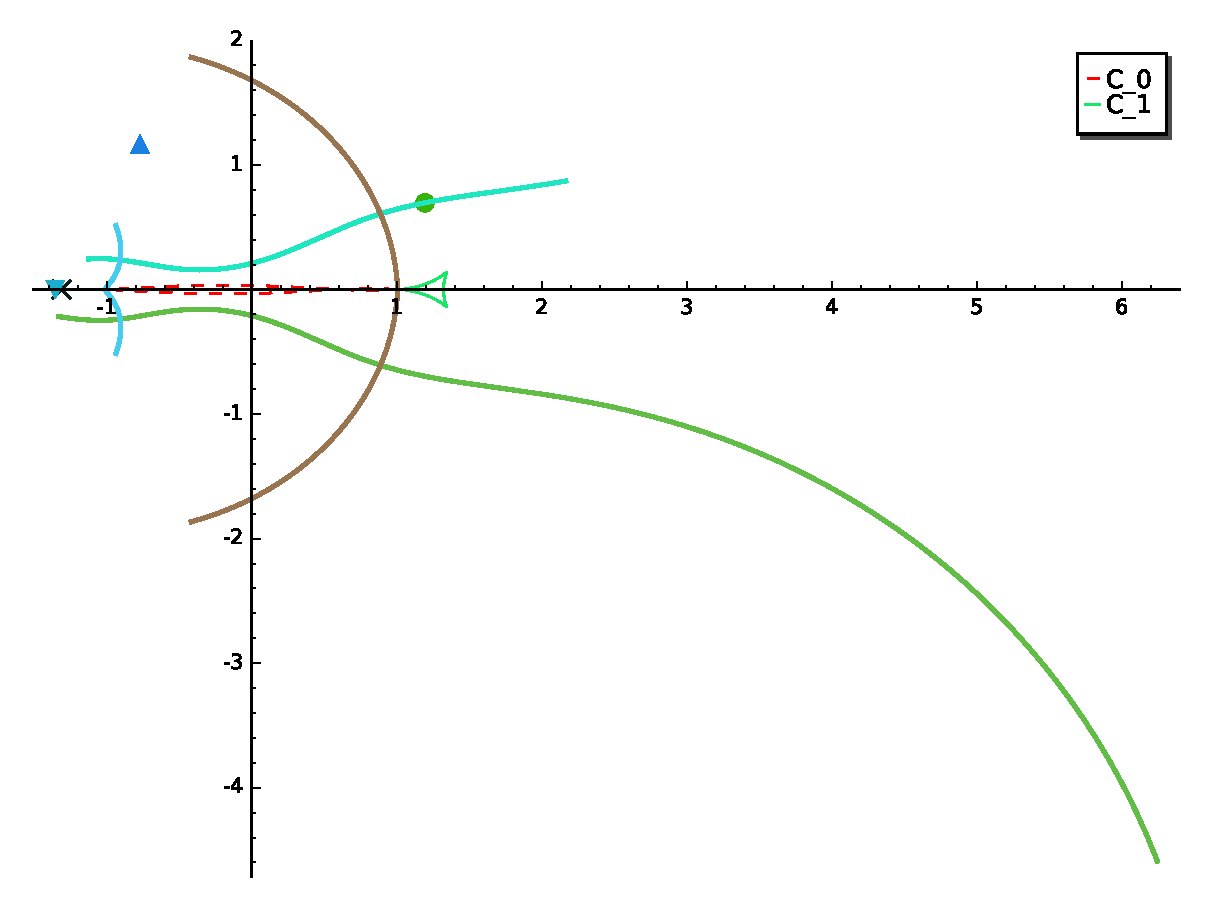
\includegraphics[width=0.5\textwidth]{zedplot.eps}
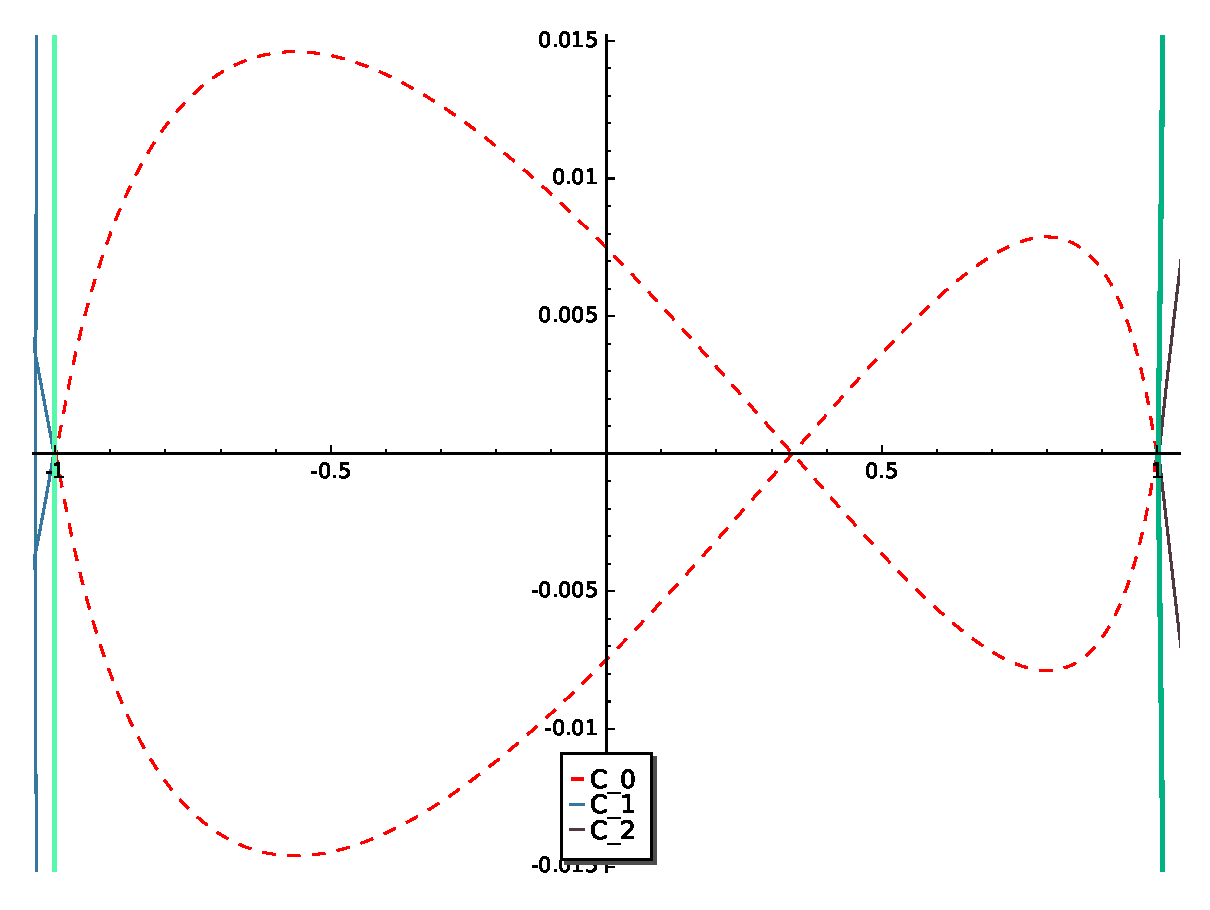
\includegraphics[width=0.5\textwidth]{zedplot_C0.eps}
\end{figure}

\newpage 
\clearpage
\section{GE2LE1}
\graphicspath{{./GE2LE1PT2/}}
\begin{figure}[!ht]
\caption{Product Threshold 3}
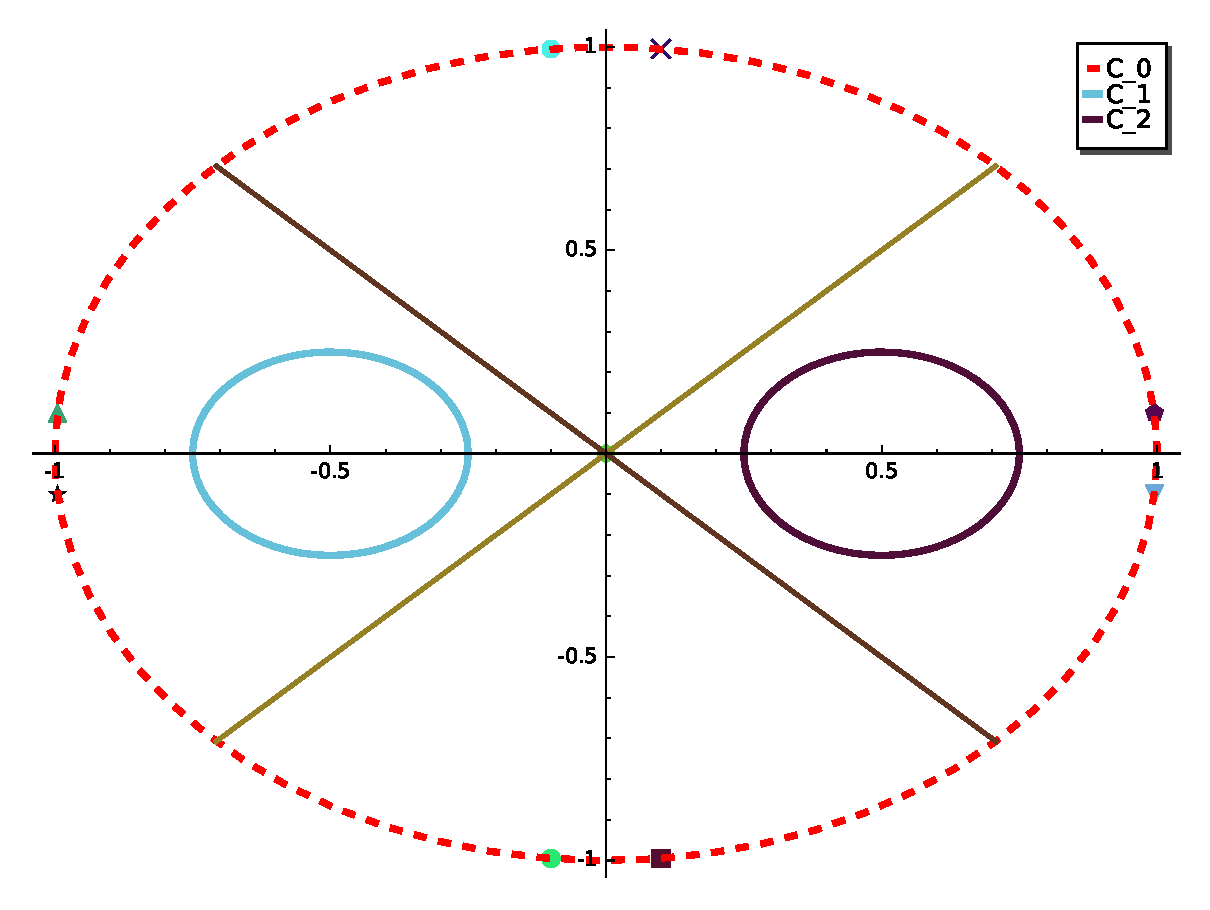
\includegraphics[width=0.5\textwidth]{circle_plot.eps}
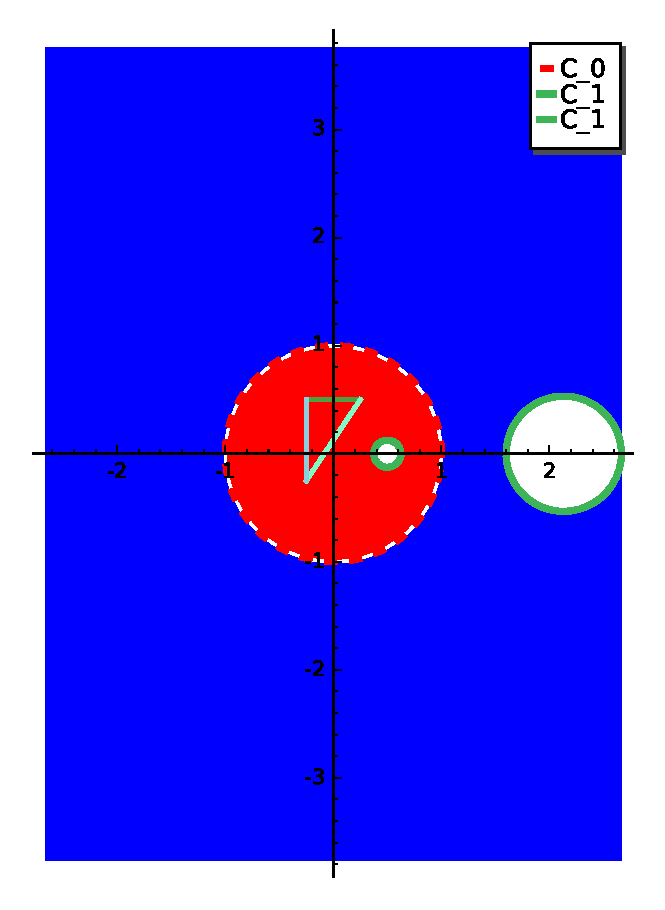
\includegraphics[width=0.5\textwidth]{Fundamental_domain.eps}
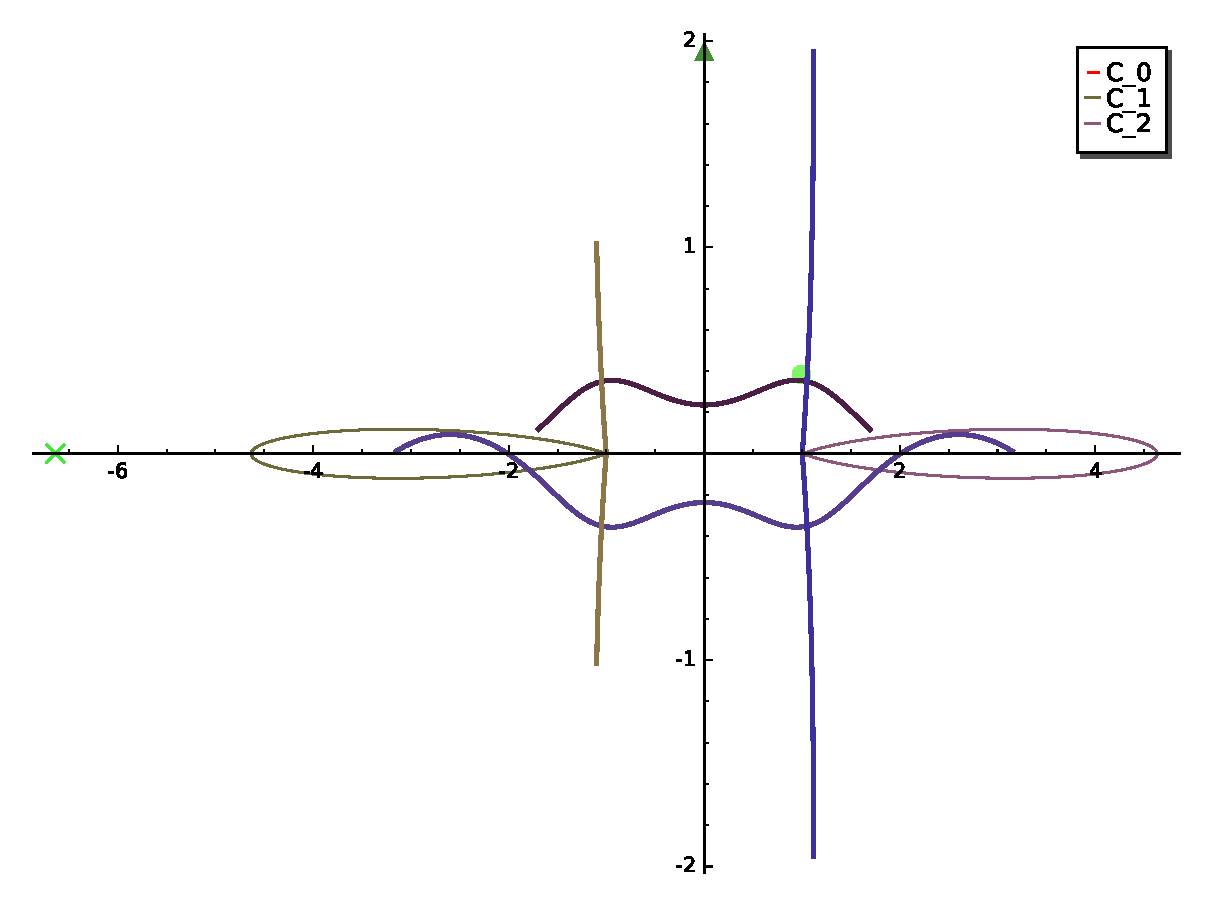
\includegraphics[width=0.5\textwidth]{zedplot.eps}
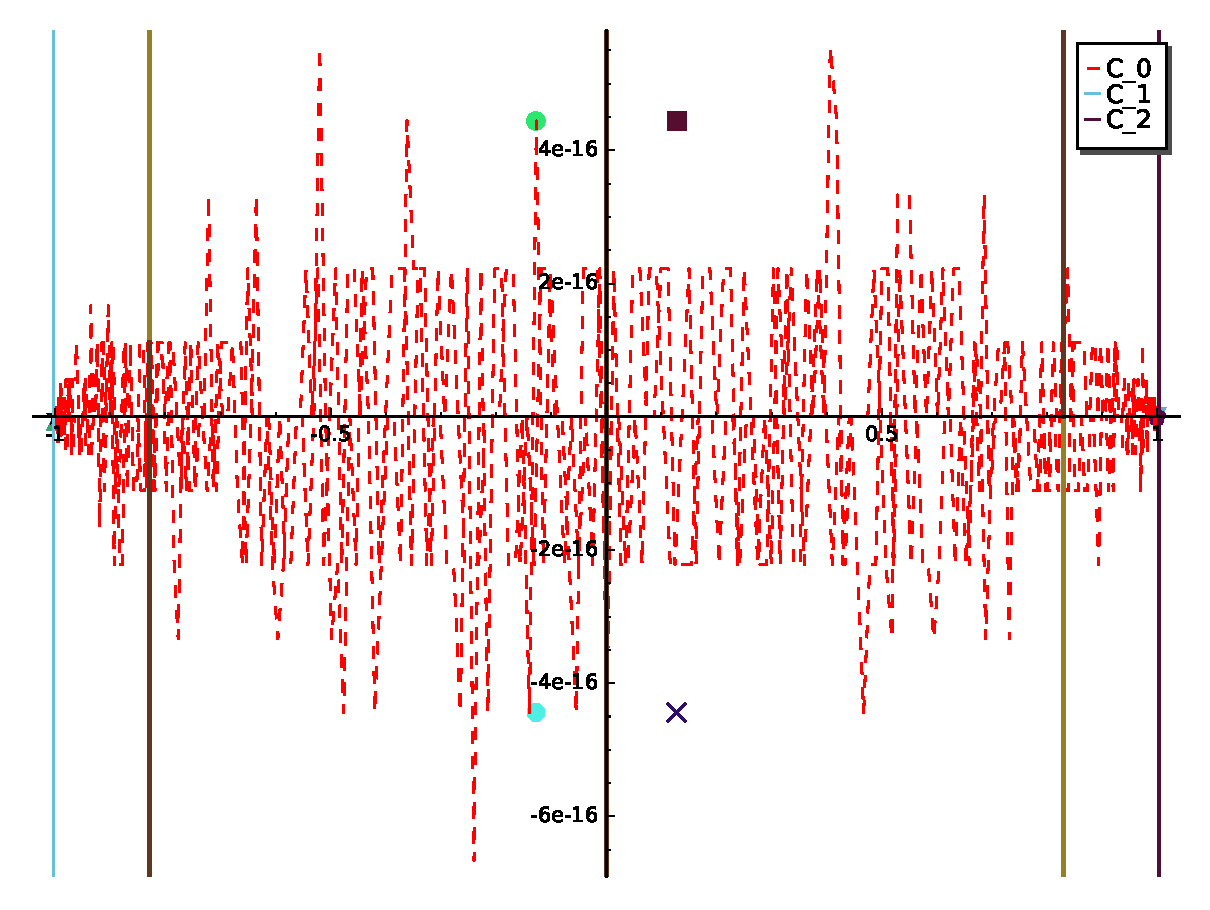
\includegraphics[width=0.5\textwidth]{zedplot_C0.eps}
\end{figure}
\graphicspath{{./GE2LE1PT3/}}
\begin{figure}[!ht]
\caption{Product Threshold 3}
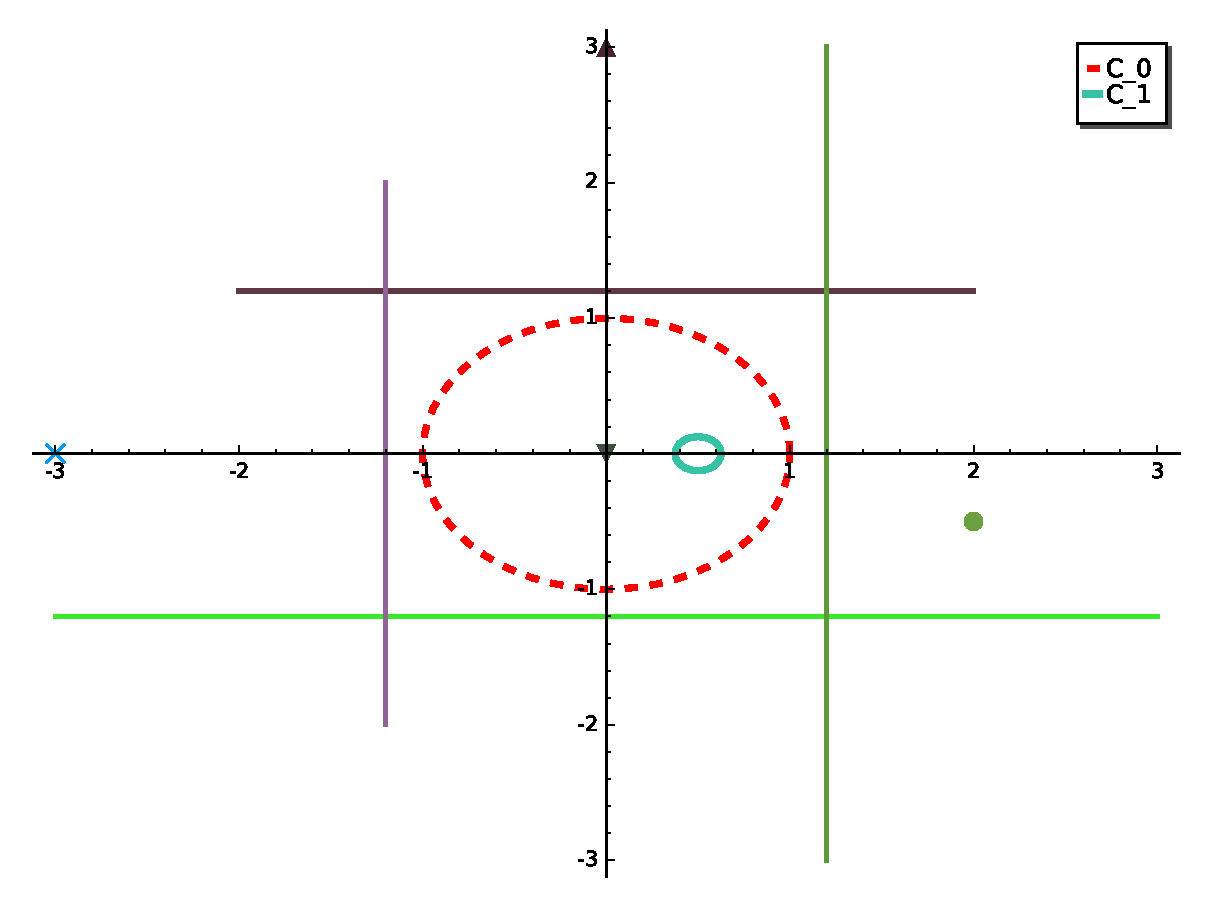
\includegraphics[width=0.5\textwidth]{circle_plot.eps}
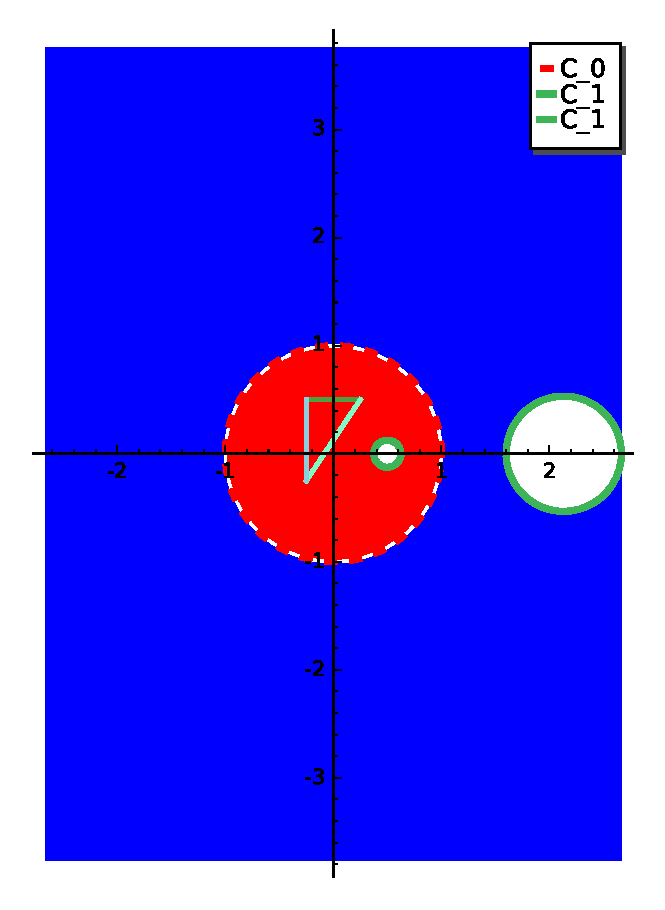
\includegraphics[width=0.5\textwidth]{Fundamental_domain.eps}
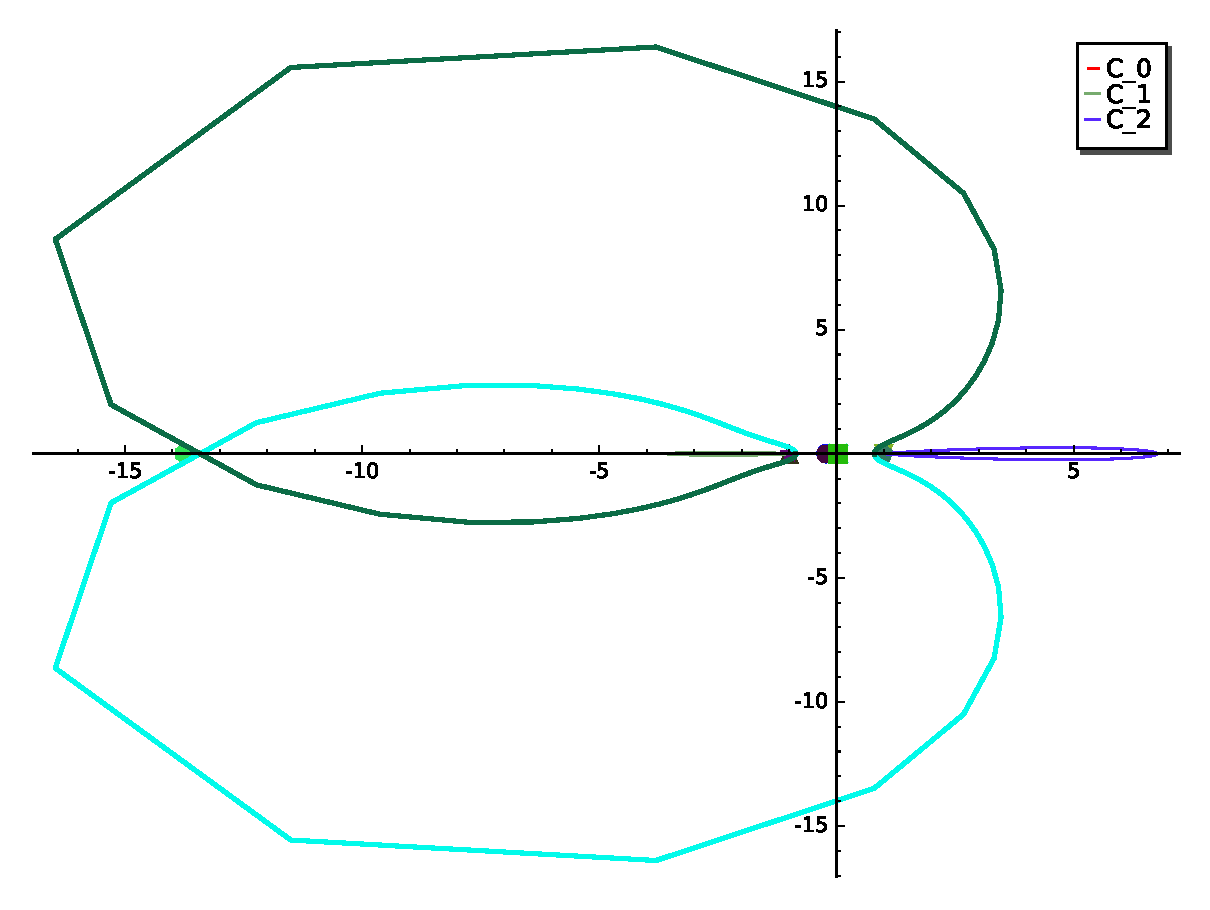
\includegraphics[width=0.5\textwidth]{zedplot.eps}
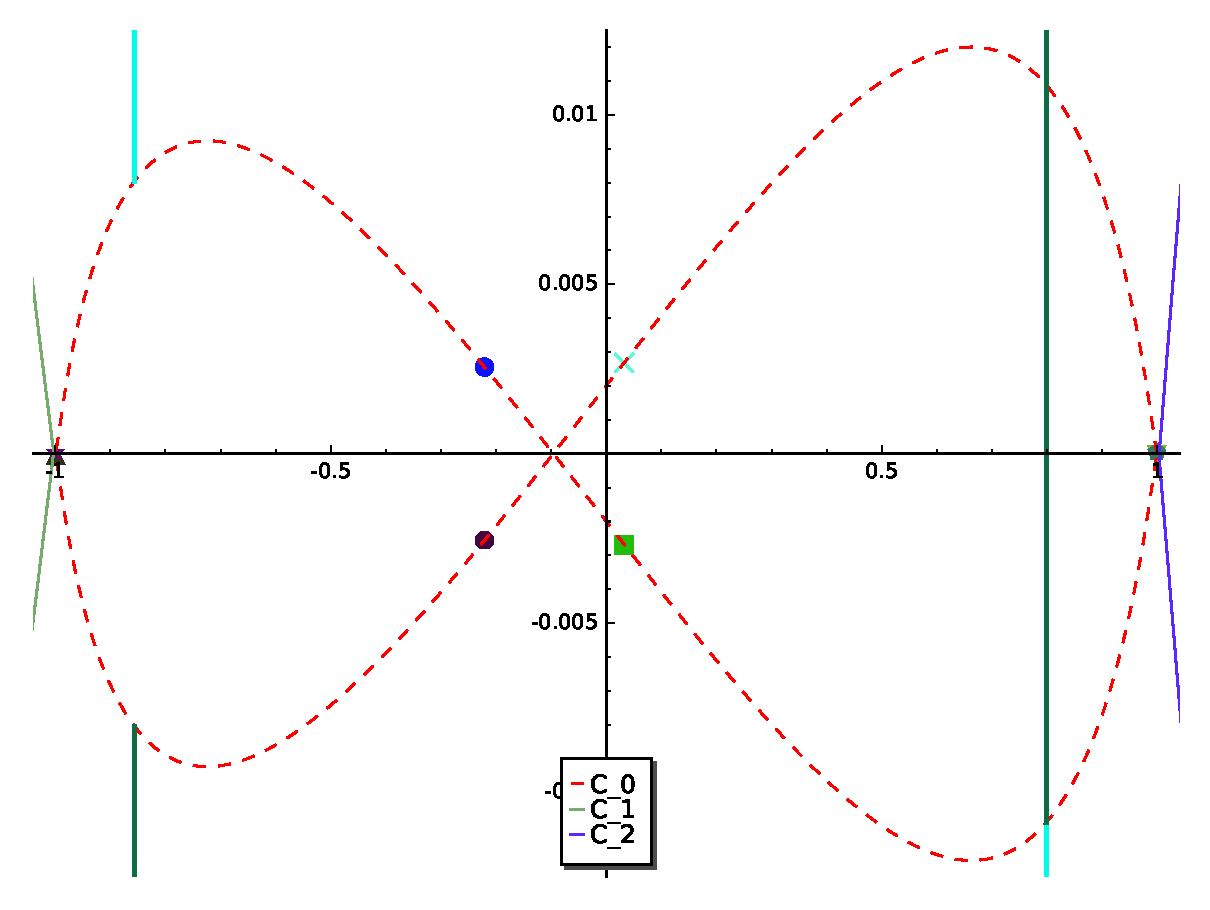
\includegraphics[width=0.5\textwidth]{zedplot_C0.eps}
\end{figure}

\graphicspath{{./GE2LE1PT4/}}
\begin{figure}
\caption{Product Threshold 4}
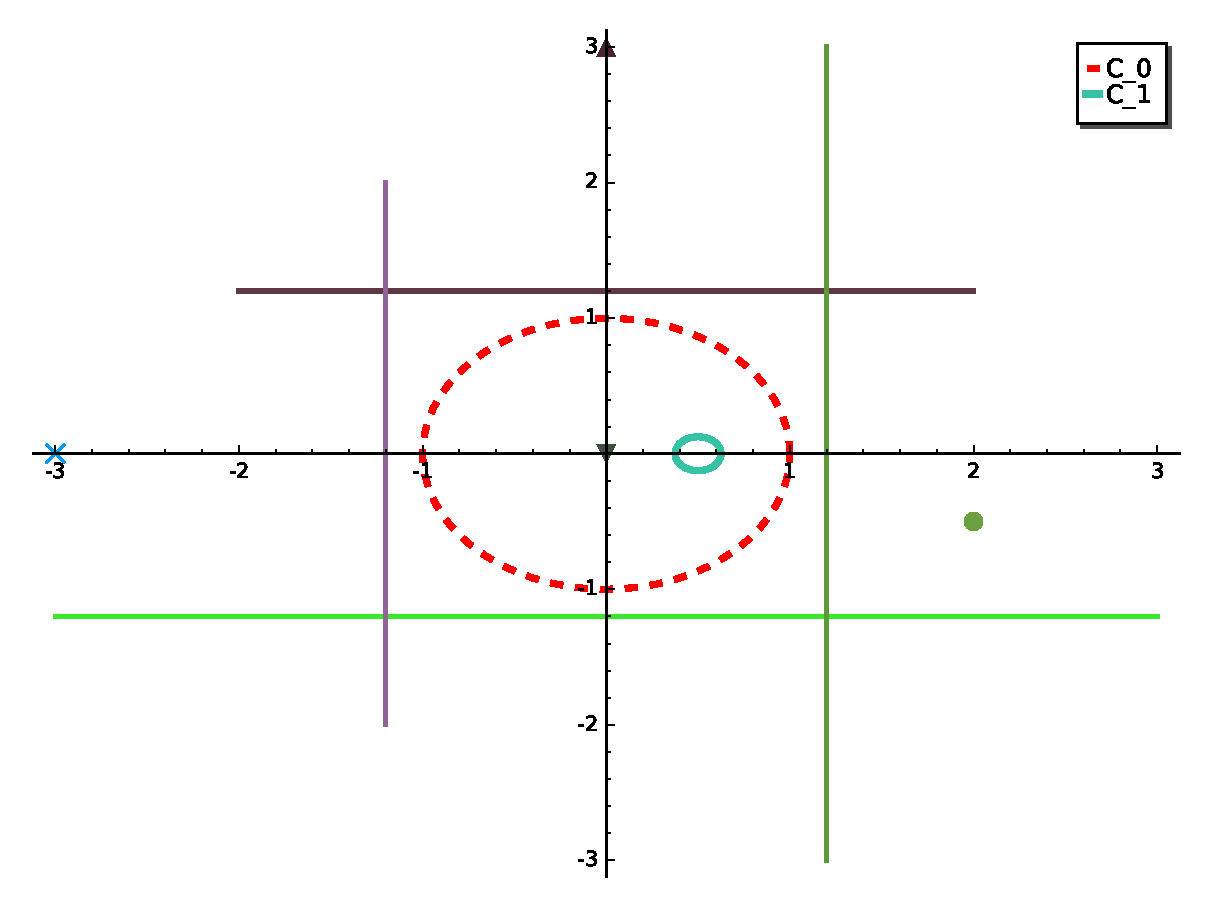
\includegraphics[width=0.5\textwidth]{circle_plot.eps}
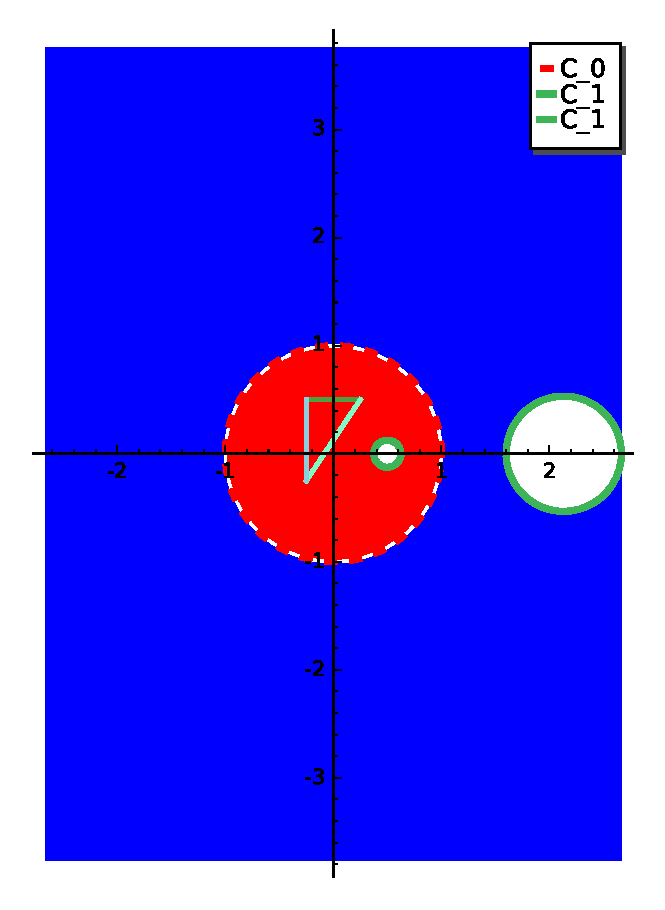
\includegraphics[width=0.5\textwidth]{Fundamental_domain.eps}
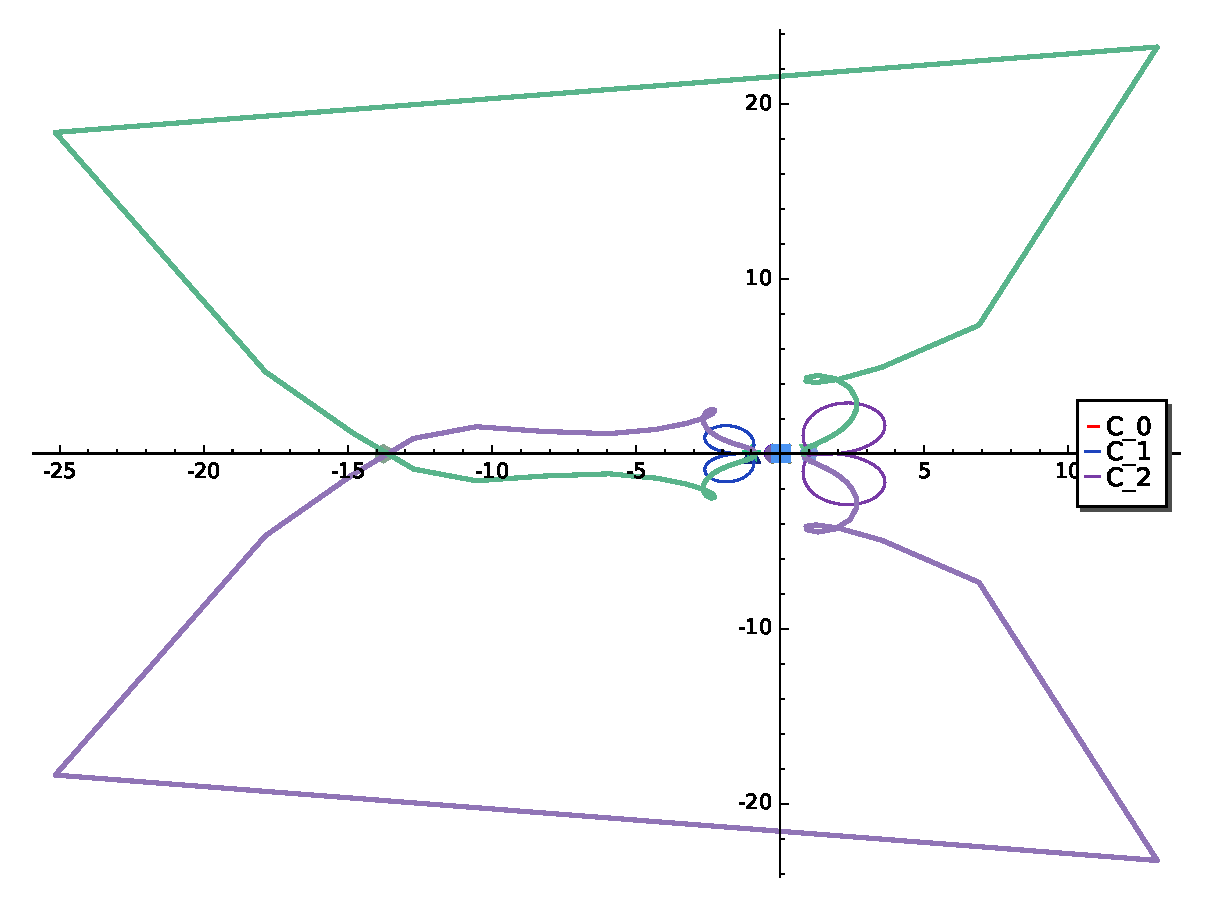
\includegraphics[width=0.5\textwidth]{zedplot.eps}
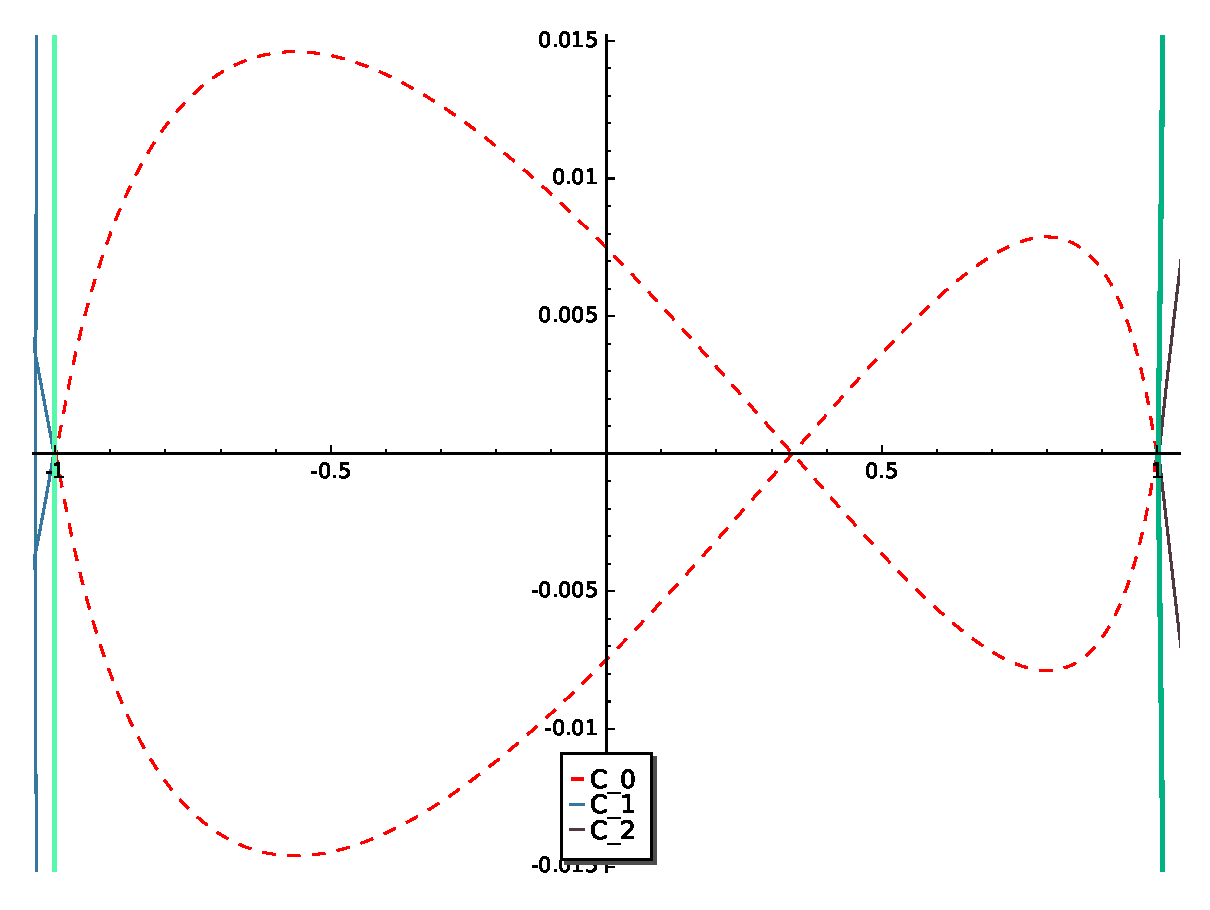
\includegraphics[width=0.5\textwidth]{zedplot_C0.eps}
\end{figure}

\graphicspath{{./GE2LE1PT5/}}
\begin{figure}
\caption{Product Threshold 5}
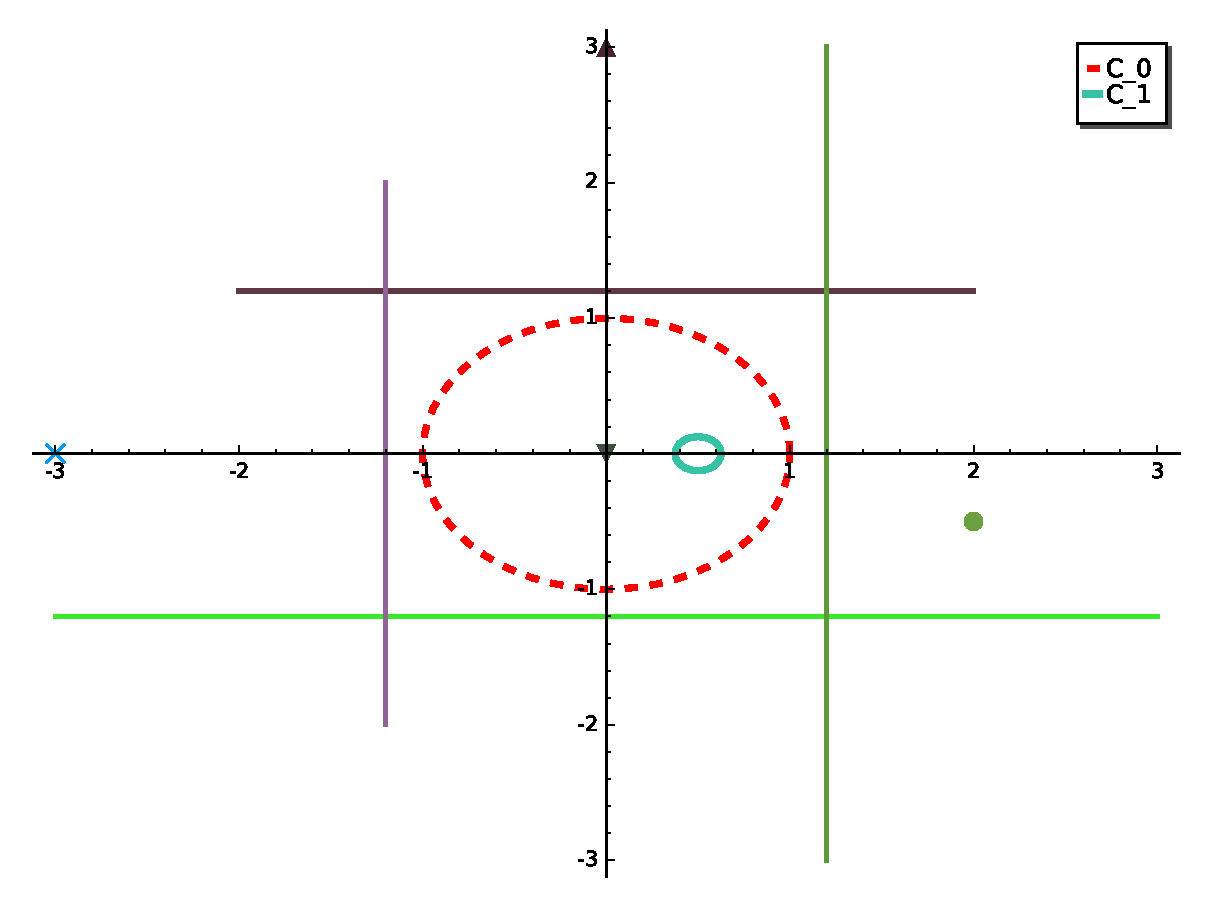
\includegraphics[width=0.5\textwidth]{circle_plot.eps}
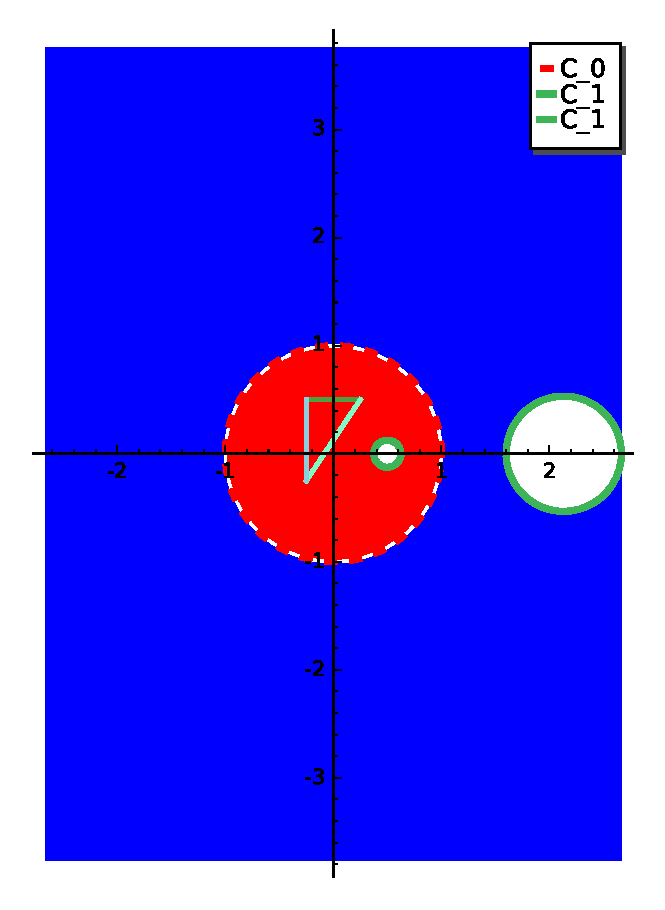
\includegraphics[width=0.5\textwidth]{Fundamental_domain.eps}
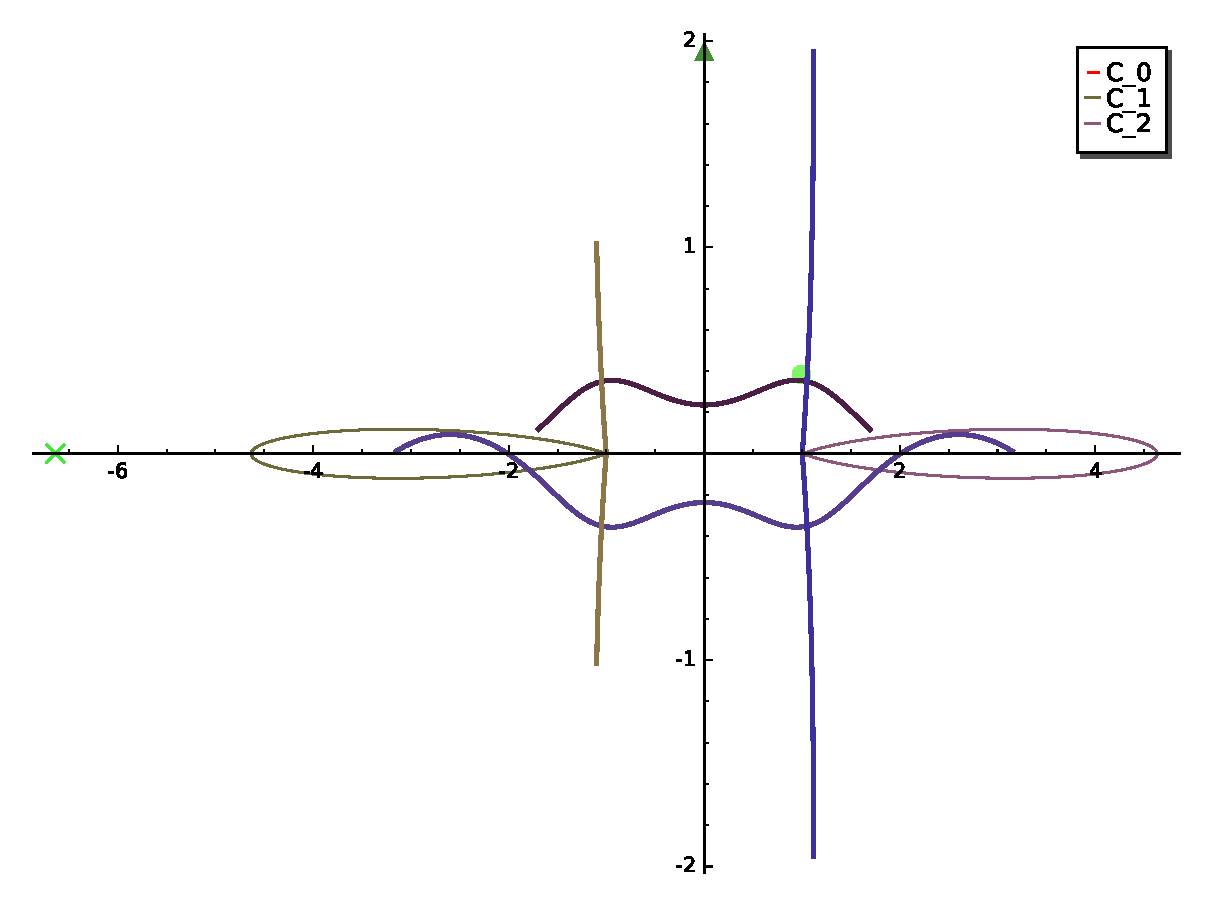
\includegraphics[width=0.5\textwidth]{zedplot.eps}
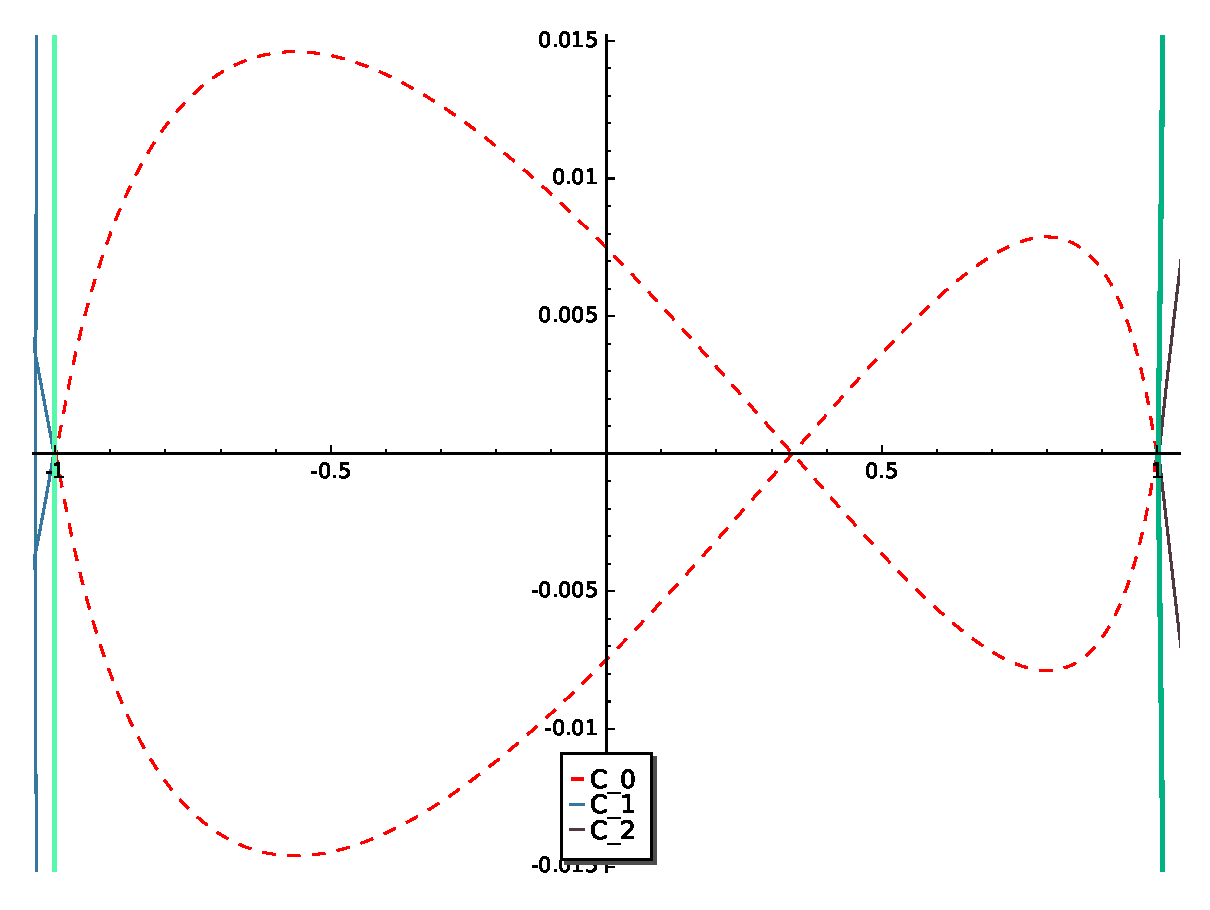
\includegraphics[width=0.5\textwidth]{zedplot_C0.eps}
\end{figure}

\end{document}
